\documentclass[a4paper,11pt]{book}

% ----- Encoding and language -----
\usepackage[utf8]{inputenc}
\usepackage[T1]{fontenc}
\usepackage[english]{babel}
\usepackage{lmodern}

% ----- General layout -----
\usepackage{geometry}
\geometry{left=2cm,right=2cm,top=2.5cm,bottom=3cm}
\setlength{\parindent}{0cm}
\renewcommand{\baselinestretch}{1.0}
\usepackage{parskip}
\usepackage{multicol}
\usepackage{afterpage}
\usepackage{fancyhdr}
\usepackage{comment}
\usepackage{abstract}
\usepackage{tocbibind}
\usepackage{eso-pic}
\usepackage{graphicx}
\usepackage{pdflscape}
\usepackage{rotating}
\usepackage{pdfpages}
\usepackage{svg}

% ----- Fonts and titles -----
\usepackage{sectsty}
\usepackage{titlesec}
\sectionfont{\fontsize{14}{15}\selectfont}
\subsectionfont{\fontsize{13}{15}\selectfont}
\titleformat{\section}[block]{\large\bfseries}{\thesection}{1em}{}
\titleformat{\subsection}[block]{\bfseries\hspace{2em}}{\thesubsection}{1em}{}
\titleformat{\subsubsection}[block]{\small\bfseries\hspace{4em}}{\thesubsubsection}{1em}{}
\titleformat{\chapter}[display]{\normalfont\huge\bfseries}{\chaptertitlename\ \thechapter}{20pt}{\Huge}
\titlespacing*{\chapter}{0pt}{0pt}{40pt}

% ----- Tables -----
\usepackage{tabularx}
\usepackage{xltabular}
\usepackage{longtable}
\usepackage{multirow, makecell}
\usepackage{nicematrix}
\usepackage{tabularray}
\usepackage{vcell}
\usepackage[table,xcdraw]{xcolor}

% ----- Cross-referencing -----
\usepackage{hyperref}
\usepackage{cleveref}
\hypersetup{
    colorlinks=true,
    linkcolor=black,
    filecolor=magenta,      
    urlcolor=cyan,
}
\newcommand{\secref}[1]{(Section \ref{#1})}
\newcommand{\ssecref}[1]{(\ref{#1})}
\newcommand{\chapref}[1]{(Chapitre \ref{#1})}
\newcommand{\figref}[1]{(Figure \ref{#1})}
\newcommand{\tabref}[1]{(Table \ref{#1})}

% ----- Listes -----
\usepackage{enumitem}
\setlist[itemize,1]{label=\textbullet}
\setlist[itemize,2]{label=$\circ$}
\newenvironment{myitemize}
{ \begin{itemize}
    \setlength{\itemsep}{0pt}
    \setlength{\parskip}{0pt}
    \setlength{\parsep}{0pt} }
{ \end{itemize} }

% ----- Code -----
\usepackage{listings}
\usepackage{color}
\definecolor{codegreen}{rgb}{0,0.6,0}
\definecolor{codegray}{rgb}{0.5,0.5,0.5}
\definecolor{codepurple}{rgb}{0.58,0,0.82}
\definecolor{backcolour}{rgb}{0.95,0.95,0.92}
\lstdefinestyle{mystyle}{
    backgroundcolor=\color{backcolour},
    commentstyle=\color{codegreen},
    keywordstyle=\color{magenta},
    numberstyle=\tiny\color{codegray},
    stringstyle=\color{codepurple},
    basicstyle=\ttfamily\footnotesize,
    breaklines=true,
    captionpos=b,
    keepspaces=true,
    numbers=left,
    numbersep=5pt,
    showstringspaces=false,
    tabsize=2
}
\lstset{style=mystyle}

% ----- Figures -----
\usepackage{caption}
\usepackage{subcaption}
\counterwithin{figure}{section}

% ----- Colors -----
\usepackage[dvipsnames]{xcolor}
\usepackage{soul}
\definecolor{green_new}{RGB}{194, 234, 229}
\definecolor{yellow_new}{RGB}{252,229,205}
\definecolor{red_new}{RGB}{244,204,204}
\definecolor{mygray}{rgb}{0.8,0.8,0.8}
\newcommand{\green}[1]{\colorbox{green_new}{#1}}
\newcommand{\yellow}[1]{\colorbox{yellow_new}{#1}}
\newcommand{\red}[1]{\colorbox{red_new}{#1}}
\newcommand{\gray}[1]{\colorbox{mygray}{#1}}

% ----- TikZ -----
\usepackage{tikz}
\usetikzlibrary{arrows,shapes,positioning,shadows,trees,decorations.markings}
\usepackage{pgf-pie}
\newcommand{\slice}[4]{
  \pgfmathparse{0.5*#1+0.5*#2}
  \let\midangle\pgfmathresult
  \draw[thick,fill=black!10] (0,0) -- (#1:1) arc (#1:#2:1) -- cycle;
  \node[label=\midangle:#4] at (\midangle:1) {};
  \pgfmathparse{min((#2-#1-10)/110*(-0.3),0)}
  \let\temp\pgfmathresult
  \pgfmathparse{max(\temp,-0.5) + 0.8}
  \let\innerpos\pgfmathresult
  \node at (\midangle:\innerpos) {#3};
}
\def\checkmark{\tikz\fill[scale=0.4](0,.35) -- (.25,0) -- (1,.7) -- (.25,.15) -- cycle;} 

% ----- Divers -----
\tolerance=1
\emergencystretch=\maxdimen
\hyphenpenalty=10000
\hbadness=10000
\newcommand\blankpage{%
    \null
    \thispagestyle{empty}%
    \addtocounter{page}{-1}%
    \newpage}

\begin{document}

\AddToShipoutPictureBG*{\includesvg{Image/IPPOG_Graphic_Charter_first.svg}}
\clearpage

% Title page
\begin{titlepage}
    \centering
    \vspace{1cm}
    \begin{figure}[h!]
        \centering
        \includesvg[width=.5\textwidth]{Image/IPPOG_logo.svg}
    \end{figure}
    \Huge\textbf{IPPOG Resources Portal\\GUIDELINES}
    \vspace{1cm}\\
    {Version 3 (31/07/25)}\par
    \vspace{2cm}
    {\Large\textbf{Hector PILLOT\footnote{Realized as part of the admin student contract of Hecotr Pillot (01/03/25 - 31/07/25)}}}\par
    \begin{center}
        \rule{0.5\linewidth}{1pt}
    \end{center}
    \normalsize
    For any question, please contact\\Claire.Adam.Bourdarios@cern.ch\\
    \vspace{2cm}
    \vfill 
    \centering
    \vspace{1cm}
\end{titlepage}

\AddToShipoutPictureBG{\includesvg{Image/IPPOG_Graphic_Charter.svg}}
\clearpage

\tableofcontents

\newpage

\chapter*{Introduction}\label{part:intro}
\addcontentsline{toc}{chapter}{\nameref{part:intro}}

The “Resource portal” was created in 2025, at the request of the HEP community during the ICHEP 2024 conference\footnote{
Education and Outreach Session @ICHEP 2024: \href{https://indico.cern.ch/event/1291157/contributions/5958376/}{https://indico.cern.ch/event/1291157/contributions/5958376/}}. It aims both to give an idea of outreach projects for the scientific community and to give a fair impression of the engagement and effort of the HEP outreach community.

The strategy for this resource portal is to serve as an online project database in which each outreach project is described in a post. We decided to start by uploading the projects presented by their owners and developers during IPPOG meetings' "success stories" sections. The idea here is to direct to a presentation by the authors themselves, possibly supplemented by a few resources\footnote{Presentation by Claire Adam @ICRC25: \href{https://indico.cern.ch/event/1258933/contributions/6475917/attachments/3105903/5509177/IPPOG-ICRC-ClaireAdam.pdf}{https://indico.cern.ch/event/1258933/contributions/6475917}}. We then enlarged it to include outreach parallel sessions of international conferences such as:
\begin{itemize}
    \item ICHEP – International Conference on High Energy Physics\footnote{ICHEP: \href{https://pos.sissa.it/cgi-bin/reader/family.cgi?code=ichep}{https://pos.sissa.it/cgi-bin/reader/family.cgi?code=ichep}}
    \item ICRC – International Cosmic Ray Conference\footnote{ICRC: \href{https://pos.sissa.it/cgi-bin/reader/family.cgi?code=icrc}{https://pos.sissa.it/cgi-bin/reader/family.cgi?code=icrc}}
    \item HEP-EPS – European Physical Society Conference on High Energy Physics\footnote{HEP-EPS: \href{https://pos.sissa.it/cgi-bin/reader/family.cgi?code=hep}{https://pos.sissa.it/cgi-bin/reader/family.cgi?code=hep}}
    \item LHCP – Large Hadron Collider Physics\footnote{LHCP: \href{https://pos.sissa.it/cgi-bin/reader/family.cgi?code=lhcp}{https://pos.sissa.it/cgi-bin/reader/family.cgi?code=lhcp}}
\end{itemize}

\bigskip

The website is built on the new CERN WordPress infrastructure\footnote{CERN WordPress infrastructure: \href{https://wordpress.docs.cern.ch/}{https://wordpress.docs.cern.ch/}}, which should replace the CERN Drupal websites from July 2025 onwards.

This document is divided into two parts. The first part (\ref{part:general}) gives a general explanation of the website and its current status (Chapter \ref{chap:context}). The second part (\ref{part:tech}) is a technical description of the website and of the upload process. Its first chapter gives an overview of the website's structure (Chapter \ref{chap:structure}), the second describes the whole automated process (Chapter \ref{chap:process}) from the database to uploading the projects on the website, and finally, the third chapter offers a visualization of the data uploaded on the website (Chapter \ref{chap:data}). The last chapter reviews useful links related to the website (Chapter \ref{chap:links}).
\part{General Description}\label{part:general}

\chapter{Context}\label{chap:context}

As of 2025, CERN made the decision to migrate its website from Drupal to WordPress\footnote{\href{https://wordpress.docs.cern.ch/}{https://wordpress.docs.cern.ch/}}. A key point about this software is the different types of content that can be created. It comes in two types: pages and posts (Section \ref{ssec:typecontent}). During the website development phase, significant attention was given to the structure of posts, ensuring easy access through a clear taxonomy (Section \ref{ssec:categorization}) and enhancing readability by pinpointing important content to emphasize (Section \ref{ssec:content}).

\section{WordPress types of content}\label{ssec:typecontent}

WordPress enables the creation of two types of content: Pages and Posts\footnote{\href{https://wordpress.com/support/post-vs-page/}{https://wordpress.com/support/post-vs-page/}}. Both display content on a website but are used for different purposes. 

\subsection*{Pages}
Pages are permanent fixtures of the site for people to access at any time. On this website, pages are typically used for the Homepage or the description of the taxonomy.

\subsection*{Posts}
Posts are individual pieces of content. They are associated with properties like date, categories, tags, keywords, or even a picture and an excerpt. On this website, posts are used for presenting outreach projects. Thanks to the post properties, each project can be efficiently categorized according to the taxonomy and sorted depending on the need.

\newpage
\section{Taxonomy of the projects}\label{ssec:categorization}

The website aims to function as an online repository for outreach projects, serving as a resource hub. Therefore, it's essential to arrange these projects, and considerable work has gone into defining a taxonomy for classifying the projects. The RDB tags list\footnote{\href{https://ippog.org/ippog-resource-database}{https://ippog.org/ippog-resource-database}} was used as a reference, but instead of focusing on resources like the previous website, this portal focuses on projects. And, as the objective of the portal changed, the taxonomy had to change as well. To define the current taxonomy, a first draft was proposed, based on various resource portals like CERN's\footnote{\href{https://home.cern/resources}{https://home.cern/resources}} or the Perimeter Institute\footnote{\href{https://resources.perimeterinstitute.ca/}{https://resources.perimeterinstitute.ca/}}. 

In the meantime, approximately 120 outreach projects were identified from presentations made during "success stories" sessions of IPPOG meetings. In these sessions, conveners share their own outreach projects in particle physics and discuss the challenges and opportunities they faced. The taxonomy was evaluated against these projects to find out if it was adjusted appropriately and to check for any categories that were either vacant or excessively filled. The classification system was further refined, with new projects being added afterward. The final taxonomy finally stabilized with 25 categories (Table \ref{tab:categories}) grouped into 4 meta-categories: 

\subsection*{Topic}
The topic refers to the main subject that the project focuses on.\newline
\textit{It can be, for example: Physics, Art, Sociology...}

\subsection*{Type}
The project type refers to the format that the project takes.\newline
\textit{It can be, for example: Book, Movie, Show...}

\subsection*{Audience}
The audience refers to the intended public, the specific group to which the project is adapted.\newline
\textit{It can be, for example: Adults, Children, Scientists...}

\subsection*{Language}
The language is a bit different from the other categories. It corresponds to the language in which projects were developed and aims to group together same-language projects in an effort to form discussion groups to help build language-specific pages and/or to collect material.

\begin{table}[h!]
    \begin{tabular}{|l|l|l|l|}
        \hline
        \textbf{Topic (5)} & \textbf{Type (8)} & \textbf{Audience (6)} & \textbf{Language (6)} \\ \hline
        Universe & Labs \& Visit Centers & Primary School (4-12 yo) & English \\ 
        Matter \& Forces & Online Resources & Educators \& Outreach Community & French \\ 
        Technology & Festivals \& Temporary Events & Secondary School (12-19 yo) & German \\ 
        Science \& Society & Open Science Projects & Broad Public & Italian \\ 
        Art Science & National Outreach Programs & University Level (19+ yo) & Portuguese \\ 
        & Books \& Publications & Scientific Community & Spanish \\ 
        & Hands on Activities &  &  \\ 
        & Games &  &  \\ \hline
    \end{tabular}
    \caption{Categories}
    \label{tab:categories}
\end{table}

\newpage
These categories allow for straightforward navigation across the resource website. However, they lack the specificity needed to locate a particular project. To address this problem, tags were developed using the same method as categories. They act as a subcategory, with each category being subdivided into several tags to enable a fine-tuned search (Fig. \ref{fig:Topics_category} \& \ref{fig:Types_category}). 

Note, however, that if every project has categories, they don't all have tags. The decision was taken to specifically mention tags only for projects that focus on a specific field. For example, a very general project about "Matter \& Force", referring to "Higgs", "Neutrinos", "Antimater" and "Nuclear physics" will only have the "Matter \& Force" category and no tags, but a project about "Matter \& Force" specifically about "Higgs" will have both the "Matter \& Force" category and "Higgs" tag.

The current state of the website, including the number of projects from each category and tag, is available in Section \ref{ssec:state}.

\section{Content choice}\label{ssec:content}

The aim of the resource portal is to provide access to the projects for all interested parties, regardless of whether they come from a scientific background or not. As such, posts had to be explicit while not being too dense. To achieve this, key information was identified as being:
\begin{itemize}
    \item The name of the projects and a general description
    \item Information about its authors and a way to contact them
    \item Status of the project
    \item Additional information
\end{itemize}

They were further developed as the following:

\subsection*{Introduction}
This section provides a summary of the project, including its name in English (and in its original language, if available) along with an image that represents it. A brief abstract is included that outlines the project's main idea without going into details. For additional information about the project, a link to the presentation given at the conference is included.

\subsection*{Information about its authors}
This section lists all authors involved in the project as well as their affiliations. There are also the affiliated IPPOG members\footnote{\href{https://ippog.org/members}{https://ippog.org/members}} or associated members\footnote{\href{https://ippog.org/associated-members}{https://ippog.org/associated-members}} and a contact, either an email or an URL leading to a contact form.

\subsection*{Status of the project}
This section gives the status of the project. It can either be "Unknown", "In preparation", "Ongoing", "Available" or "Done". As the status is subject to change, the date of the most recent update of the post is included.

\subsection*{Additional information}
This section compiles supplementary documents and links pertinent to the project. This generally include websites, presentations from other conferences, or academic papers.

\newpage
\section{Current state of the Website}\label{ssec:state}

At the moment this document is written, 121 projects have been posted on the website. Statistics regarding the affiliated IPPOG (associated) members, topics and types were produced.

\subsection*{Affiliated IPPOG (associated) members}
The representation of IPPOG members is noticeably unbalanced (Fig. \ref{fig:members}), with Germany and Italy being the most represented countries, followed by France and the United States of America, which conduct extensive outreach activities through Netzwerk Teilchenwelt, INFN, IN2P3, and QuarkNet. Major collaborations such as ATLAS and ALICE, along with CERN, also make significant contributions due to their larger scale. But most members have close to no outreach projects listed on the website. Developing language discussion groups could help reduce this gap.

A difficulty here is that the choice was made that only content presented in a conference or meeting would be uploaded on the website. This choice enables the use of a short abstract, complemented by the slides from the outreach session in which it was presented. This also guarantees the quality of the projects, as it was presented during big meetings. The problem, however, is that such outreach sessions are limited during conferences. Additionally, not all conferences offer their own outreach sessions, and some have only recently introduced them. This greatly reduces the available projects from some parts of the world.

\subsection*{Topics}
Among the covered topics, "Matter \& Force" is the most represented, with its subtopic "Standard model of elementary particles" (Fig. \ref{fig:topics}) which is no wonder, as it is the main focus of the outreach group. Three subtopics were left even though empty: "Machine learning", "Civil Engineering \& Construction" and "Cryogeny, Magnet \& Supraconductors", as they remain pertinent topics, but they could be removed if no related outreach projects are added.  

\subsection*{Types}
There are many different types of outreach projects, and this meta-category aims to demonstrate their full diversity (Fig. \ref{fig:types}). In this scenario, the "Festival" is the subtopic that appears most frequently. This is because outreach activities like demonstrations, visits, or even games tend to be used during temporary events like science fairs. As such, it is not the activity or visit that is presented during outreach sessions, but the festival in which it was used. 

Another issue is that speakers often give an overview of what their laboratory, experiment, or country did, rather than focusing on individual projects. This results in the presentation turning into a broad overview, lacking sufficient details to upload several projects onto the website. The solution found was to introduce the subtopics "Experiment" and "Laboratory" projects, as well as the topic "National outreach program" which has no subtopics.

\begin{figure}[p]
    \centering
    \includesvg[width=.7\linewidth,inkscapelatex=false]{Image/Context/Topics_category.svg}
    \caption{Categorization of Topics}
    \label{fig:Topics_category}
\end{figure}


\begin{figure}[p]
    \centering
    \includesvg[width=.6\linewidth,inkscapelatex=false]{Image/Context/Types_category.svg}
    \caption{Categorization of Types}
    \label{fig:Types_category}
\end{figure}

\begin{figure}
    \centering
    \includesvg[width=\linewidth]{Image/Context/Related_members.svg}
    \caption{Related members data}
    \label{fig:members}
\end{figure}

\begin{figure}
    \centering
    \includesvg[width=\linewidth]{Image/Context/topics.svg}
    \caption{Topics data}
    \label{fig:topics}
\end{figure}

\begin{figure}
    \centering
    \includesvg[width=\linewidth]{Image/Context/types.svg}
    \caption{Types data}
    \label{fig:types}
\end{figure}
\part{Technical Description}\label{part:tech}

\chapter{Website's Structure}\label{chap:structure}

This section will describe the different parts of the website, from the Home page (Sec. \ref{fig:home_page}) and its Menu (Sec. \ref{sec:structure_menus}) leading to the Meta-category (Sec. \ref{sec:structure_metacategories}) and Category (Sec. \ref{sec:structure_categories}) pages (with the special case of the Language category (Sec. \ref{sec:structure_language}). Then the section will describe the Posts (Sec. \ref{sec:structure_post}) and the pages generated automatically by its tags and categories (Sec. \ref{sec:structure_auto}) and will finish by explaining the General Information menu (Sec. \ref{sec:structure_genaralinfo}).

\section{Home page}\label{sec:structure_home_page}

The home page\footnote{Home page: \href{https://ippog-resources-portal.web.cern.ch/}{https://ippog-resources-portal.web.cern.ch/}} is the first page the user gets to. It aims to present the website and redirect to the main pages of the website. A screenshot is available in Figure \ref{fig:home_page}.

\subsection*{a. Home banner}
[Cover block] including the logo of the IPPOG Collaboration with a catchphrase "Explore the foundations of the universe!" over a picture of students participating in International Physics Masterclass.

\subsection*{b. Title}
[H1 Title block]: "Presenting Particle Physics Outreach Projects".

\subsection*{c. Presentation}
[Paragraph block] presenting the website.

\subsection*{d. Meta-Categories}
[Paragraph block] introducing the categories followed with [Buttons block] leading to the meta-categories pages nested within [Cover block] in a [Columns block].

\subsection*{e. Latest entries}
[Title H2] Block followed by a [News block]\footnote{The News block is a CERN customized Query Loop displaying posts and allowing the filtering per categories and/or tags. The choice was made to display the image, title, tags and excerpt of posts.} displaying the 3 latest articles uploaded. Note that it is possible to force the displayed articles as their uploaded date can be updated.

\subsection*{f. Footpage banner}
[Cover block] following the IPPOG color chart.

\begin{figure}[p]
    \centering
    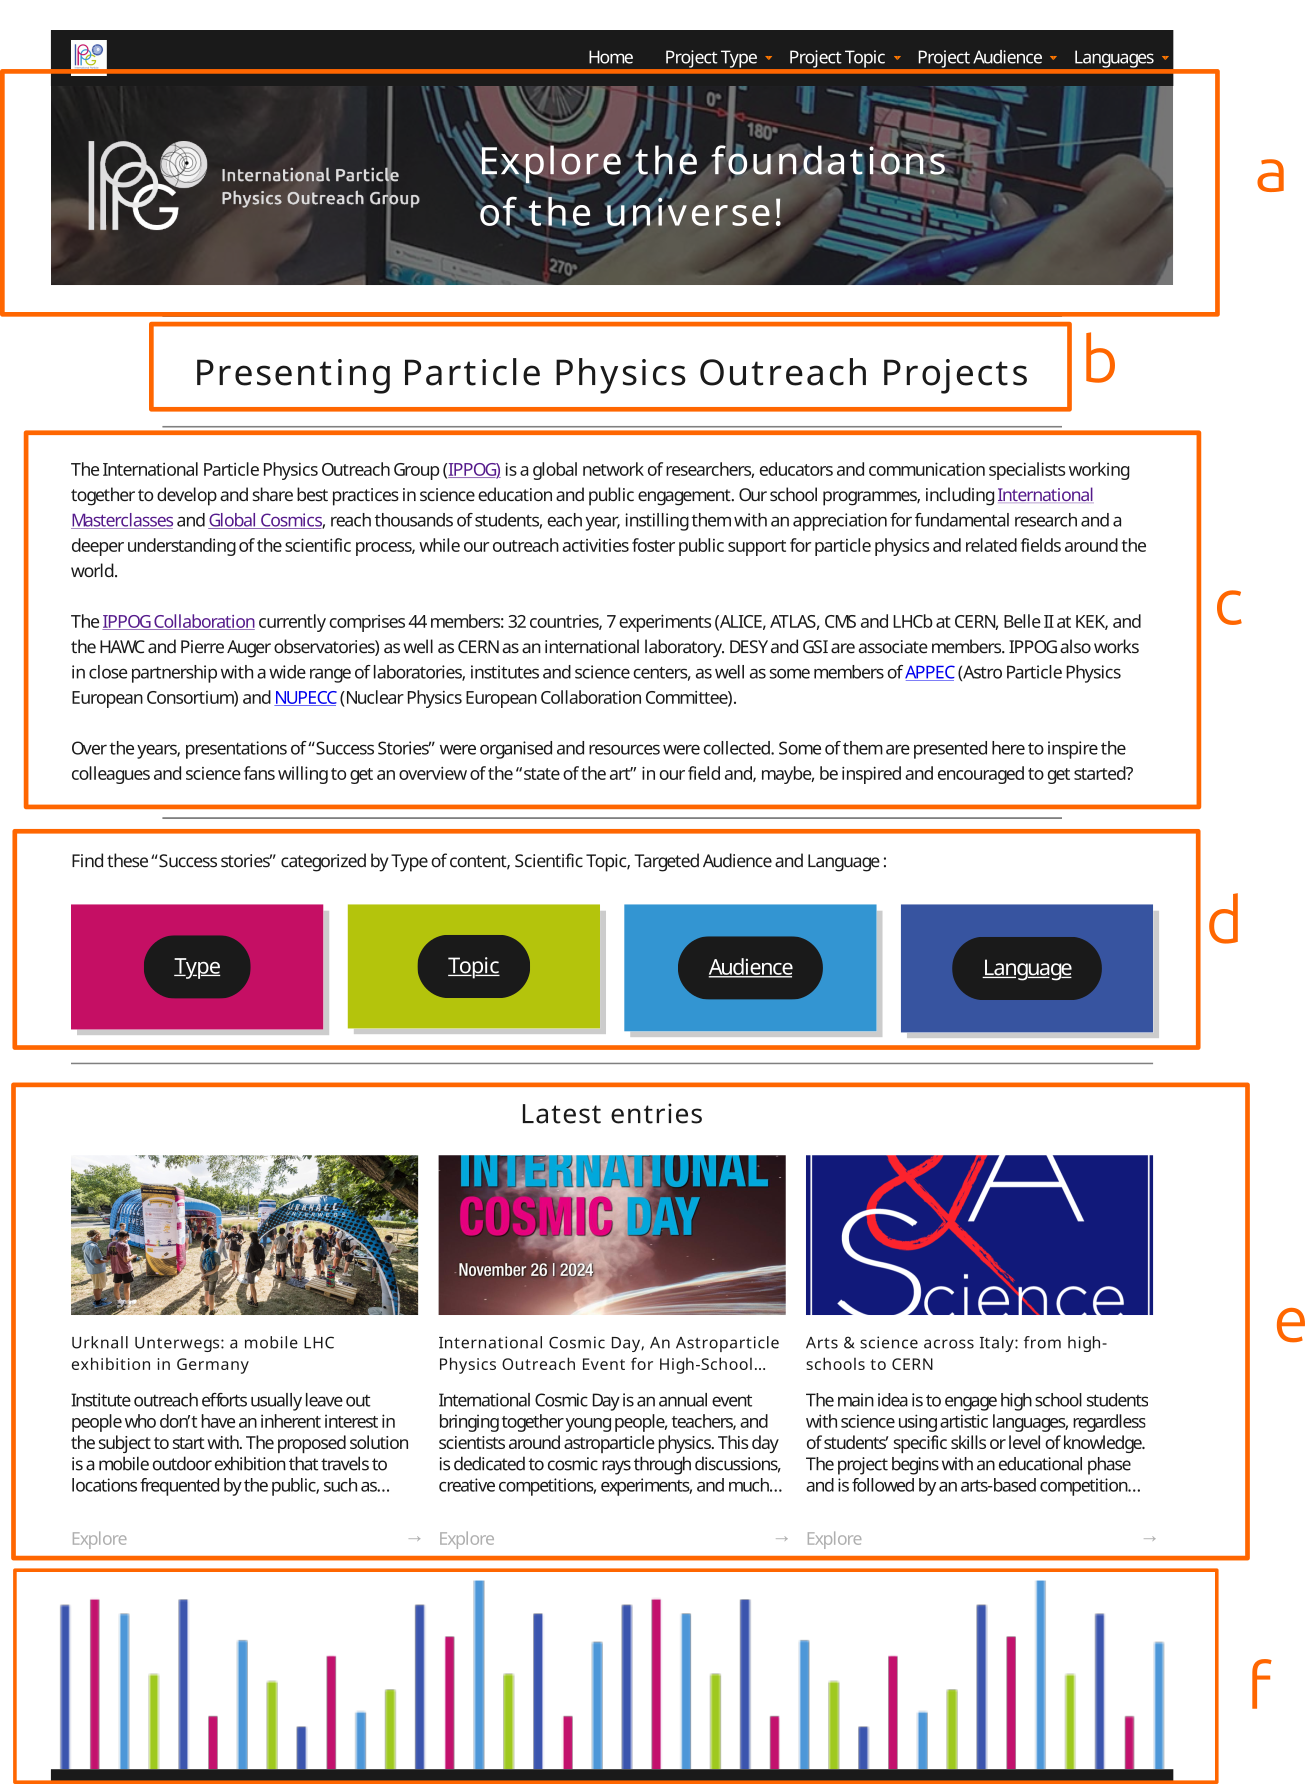
\includegraphics[width=\linewidth]{Image/Architecture/home_page.png}
    \caption{Website Home page}
    \label{fig:home_page}
\end{figure}

\newpage
\section{Menus}\label{sec:structure_menus}

Menus can be displayed in 2 locations: 
\begin{itemize}
    \item Header Navigation: at the top of the website
    \item Footer Navigation: at the bottom of the website, the footer is separated into 3 columns
\end{itemize}

\bigskip 

The website is using 3 menus (Fig. \ref{fig:menus}): 

\subsection*{a. CERN \& You}
This is the classic CERN menu displayed in all CERN websites. It is not displayed at the moment because it is not relevant for the collaboration.
/!\textbackslash \ It may automatically come back when the WordPress structure is updated.

\subsection*{b. General Information}
This menu gives further information about IPPOG and the website. 
\begin{itemize}
    \item A first link "Custom Link Brought to you by the IPPOG collaboration, on behalf of the Particle Physics outreach community." leads to the FAQ (Section \ref{ssec:structure_FAQ}),
    \item The second link "Further details on the categorization." leads to the explanation of the tags (Section \ref{ssec:structure_Categorization}).
\end{itemize}

\subsection*{c. Main Navigation}
The main navigation menu includes links to: 
\begin{itemize}
    \item the Home page (Sec. \ref{sec:structure_home_page})
    \item the different pages related to meta-categories: Project Type / Project Topic / ... (Sec. \ref{sec:structure_metacategories}). By passing the mouse over the categories name, the user can make a scroll-down menu, detailing the different category's pages: Universe / Matter \& Forces / ... (Sec. \ref{sec:structure_categories}).
\end{itemize}

\begin{figure}[p]
    \centering
    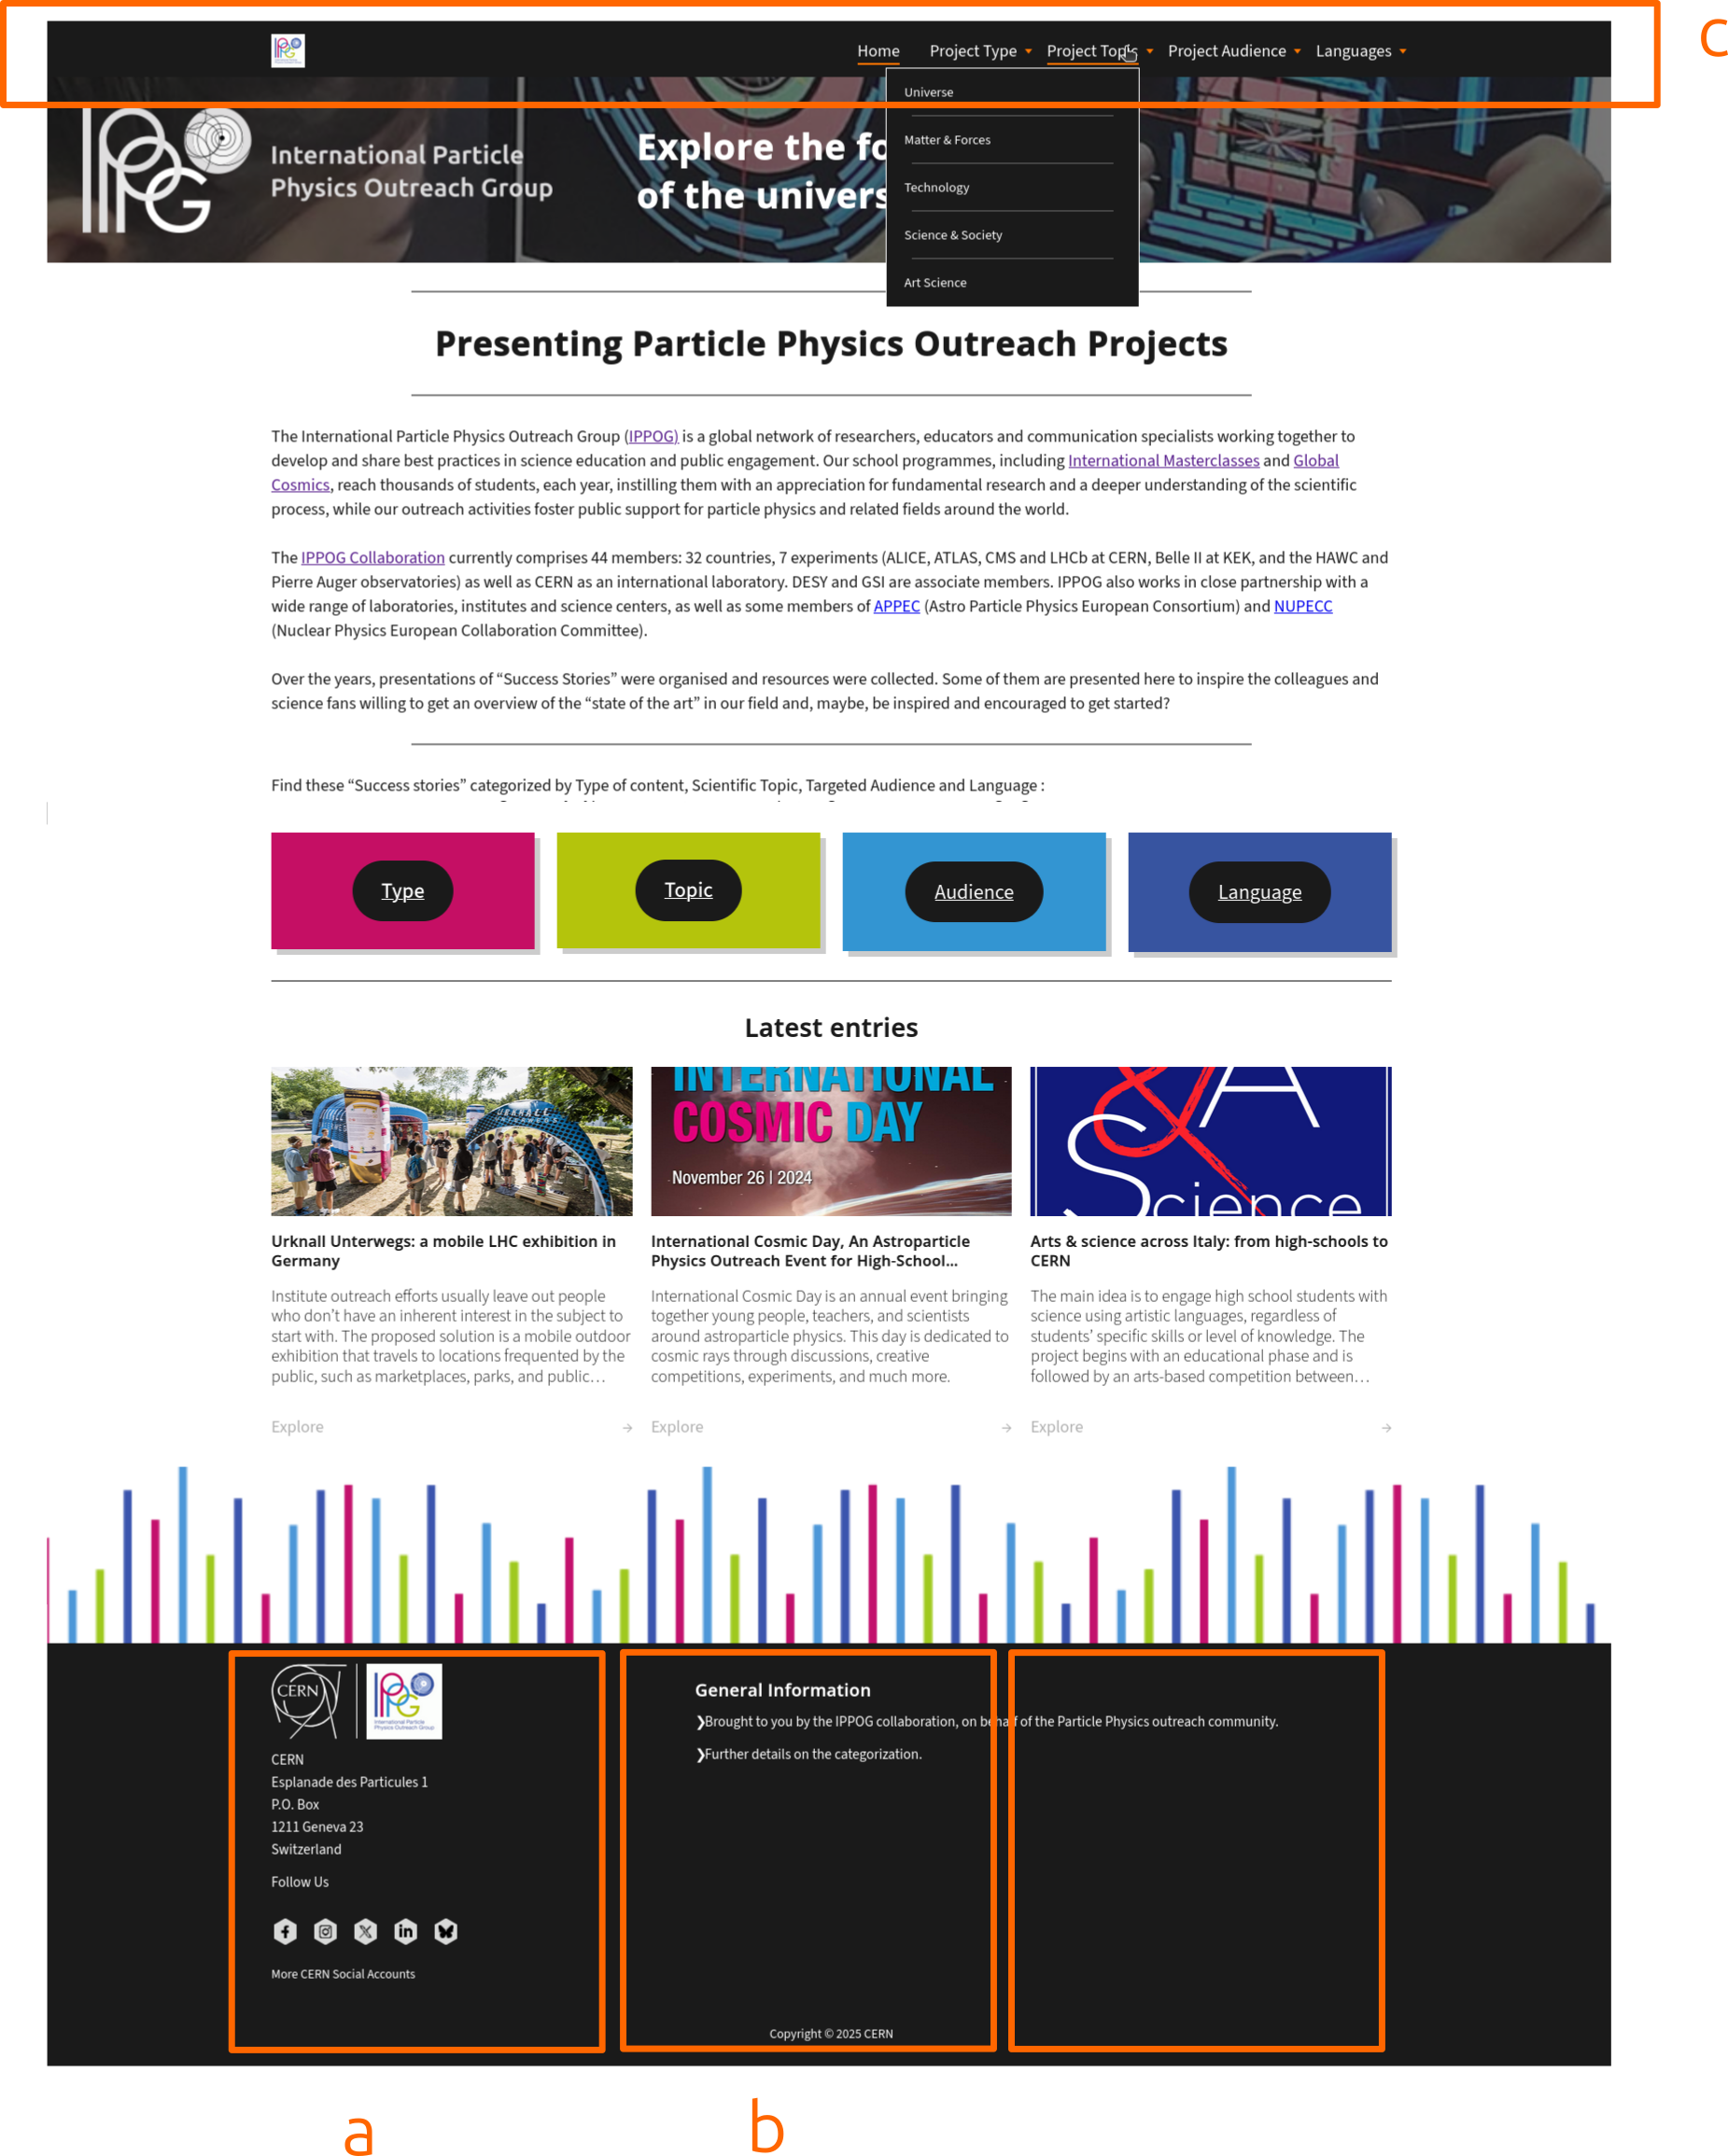
\includegraphics[width=\linewidth]{Image/Architecture/menus.png}
    \caption{Website menus}
    \label{fig:menus}
\end{figure}

\newpage
\section{Meta-Categories pages}\label{sec:structure_metacategories}

The Meta-Categories pages (Fig. \ref{fig:structure_metacategory}) display all categories related to the meta-category and the last three projects uploaded for each category.

\subsection*{a. IPPOG color chart}
[Cover block] including one of the colors of the IPPOG's color chart.

\subsection*{b. Title}
[H1 Title block]: Either "Project Type" / "Project Topic" / "Project Audience".

\subsection*{c. List of categories}
[Buttons block] leading to the categories pages nested within [Cover block] in a [Columns block].

\subsection*{d. Latest updated projects for each category}
[Group block] For each category\footnote{Except for the "Language" meta-category that doesn't have this part.}. The block contains: 
\begin{itemize}
    \item a [Cover block] including one of the colors of the IPPOG's color chart,
    \item a [H2 Title block] "Latest projects for" followed by the name of the category,
    \item a [Paragraph block] introducing the category,
    \item a [News block] displaying the 3 latest articles uploaded in the relative category.
\end{itemize}

\begin{figure}[p]
    \centering
    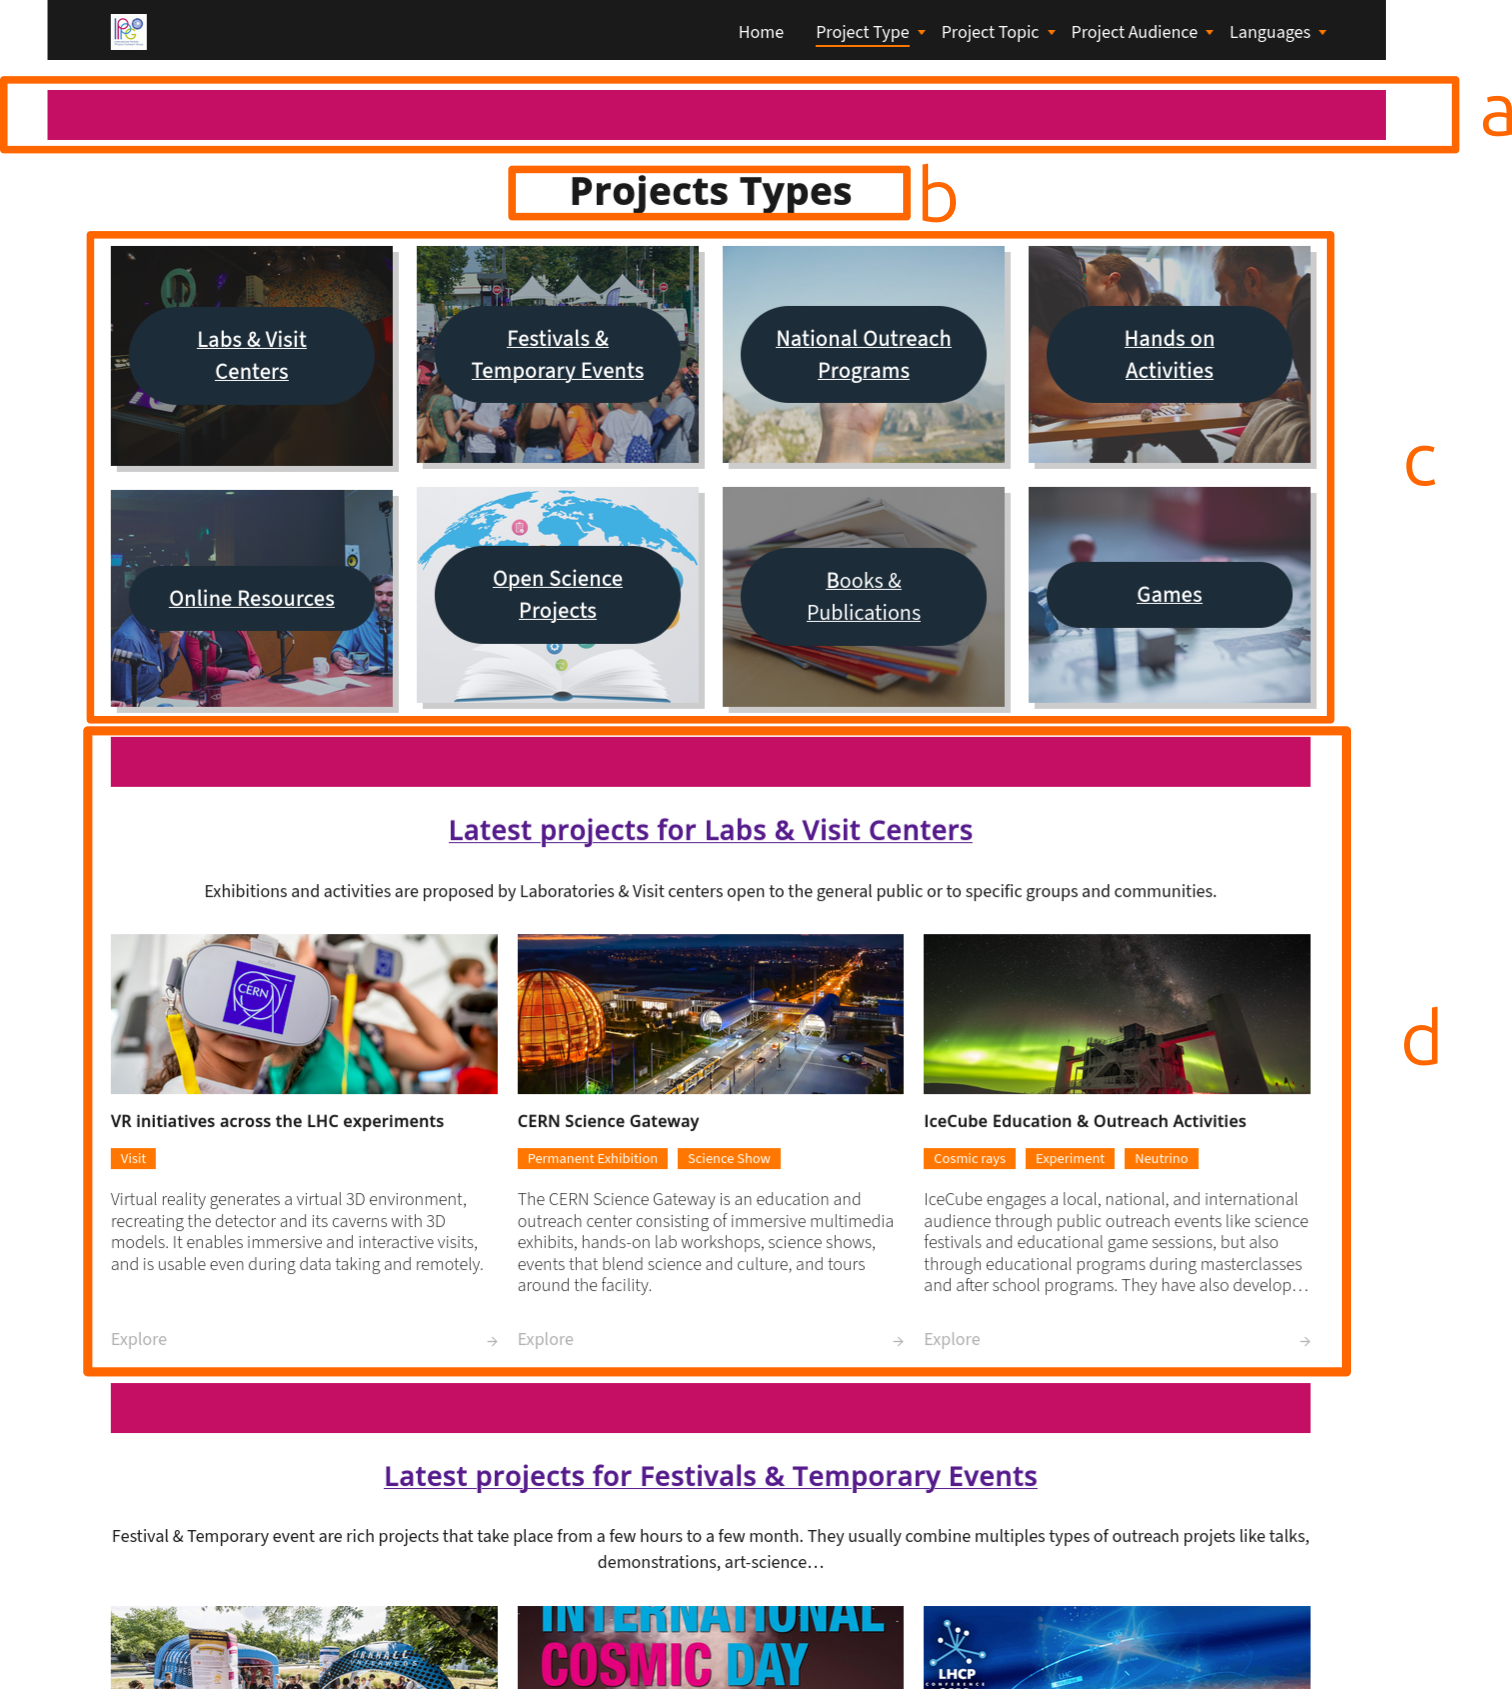
\includegraphics[width=\linewidth]{Image/Architecture/structure_types.png}
    \caption{Meta-categories pages (example of the "Projects Types" page)}
    \label{fig:structure_metacategory}
\end{figure}

\newpage

\section{Categories pages}\label{sec:structure_categories}

The Categories pages (Fig. \ref{fig:structure_category}) display all projects related to the category. The "Language" categories are a bit different and will be developed in more details in Sec. \ref{sec:structure_language}.

\subsection*{a. Category's banner}
[Cover block] including a [H1 Title block] with the name of the Category over a picture illustrating it.

\subsection*{b. Introduction}
[Paragraph block] introducing the category.

\subsection*{c. Tags}
[Paragraph block] introducing the tags followed by [Buttons block] leading to the automatically produced tags pages (Sec. \ref{sec:structure_auto})

\subsection*{d. Projects}
[News block] displaying all projects with the related category.

\begin{figure}[p]
    \centering
    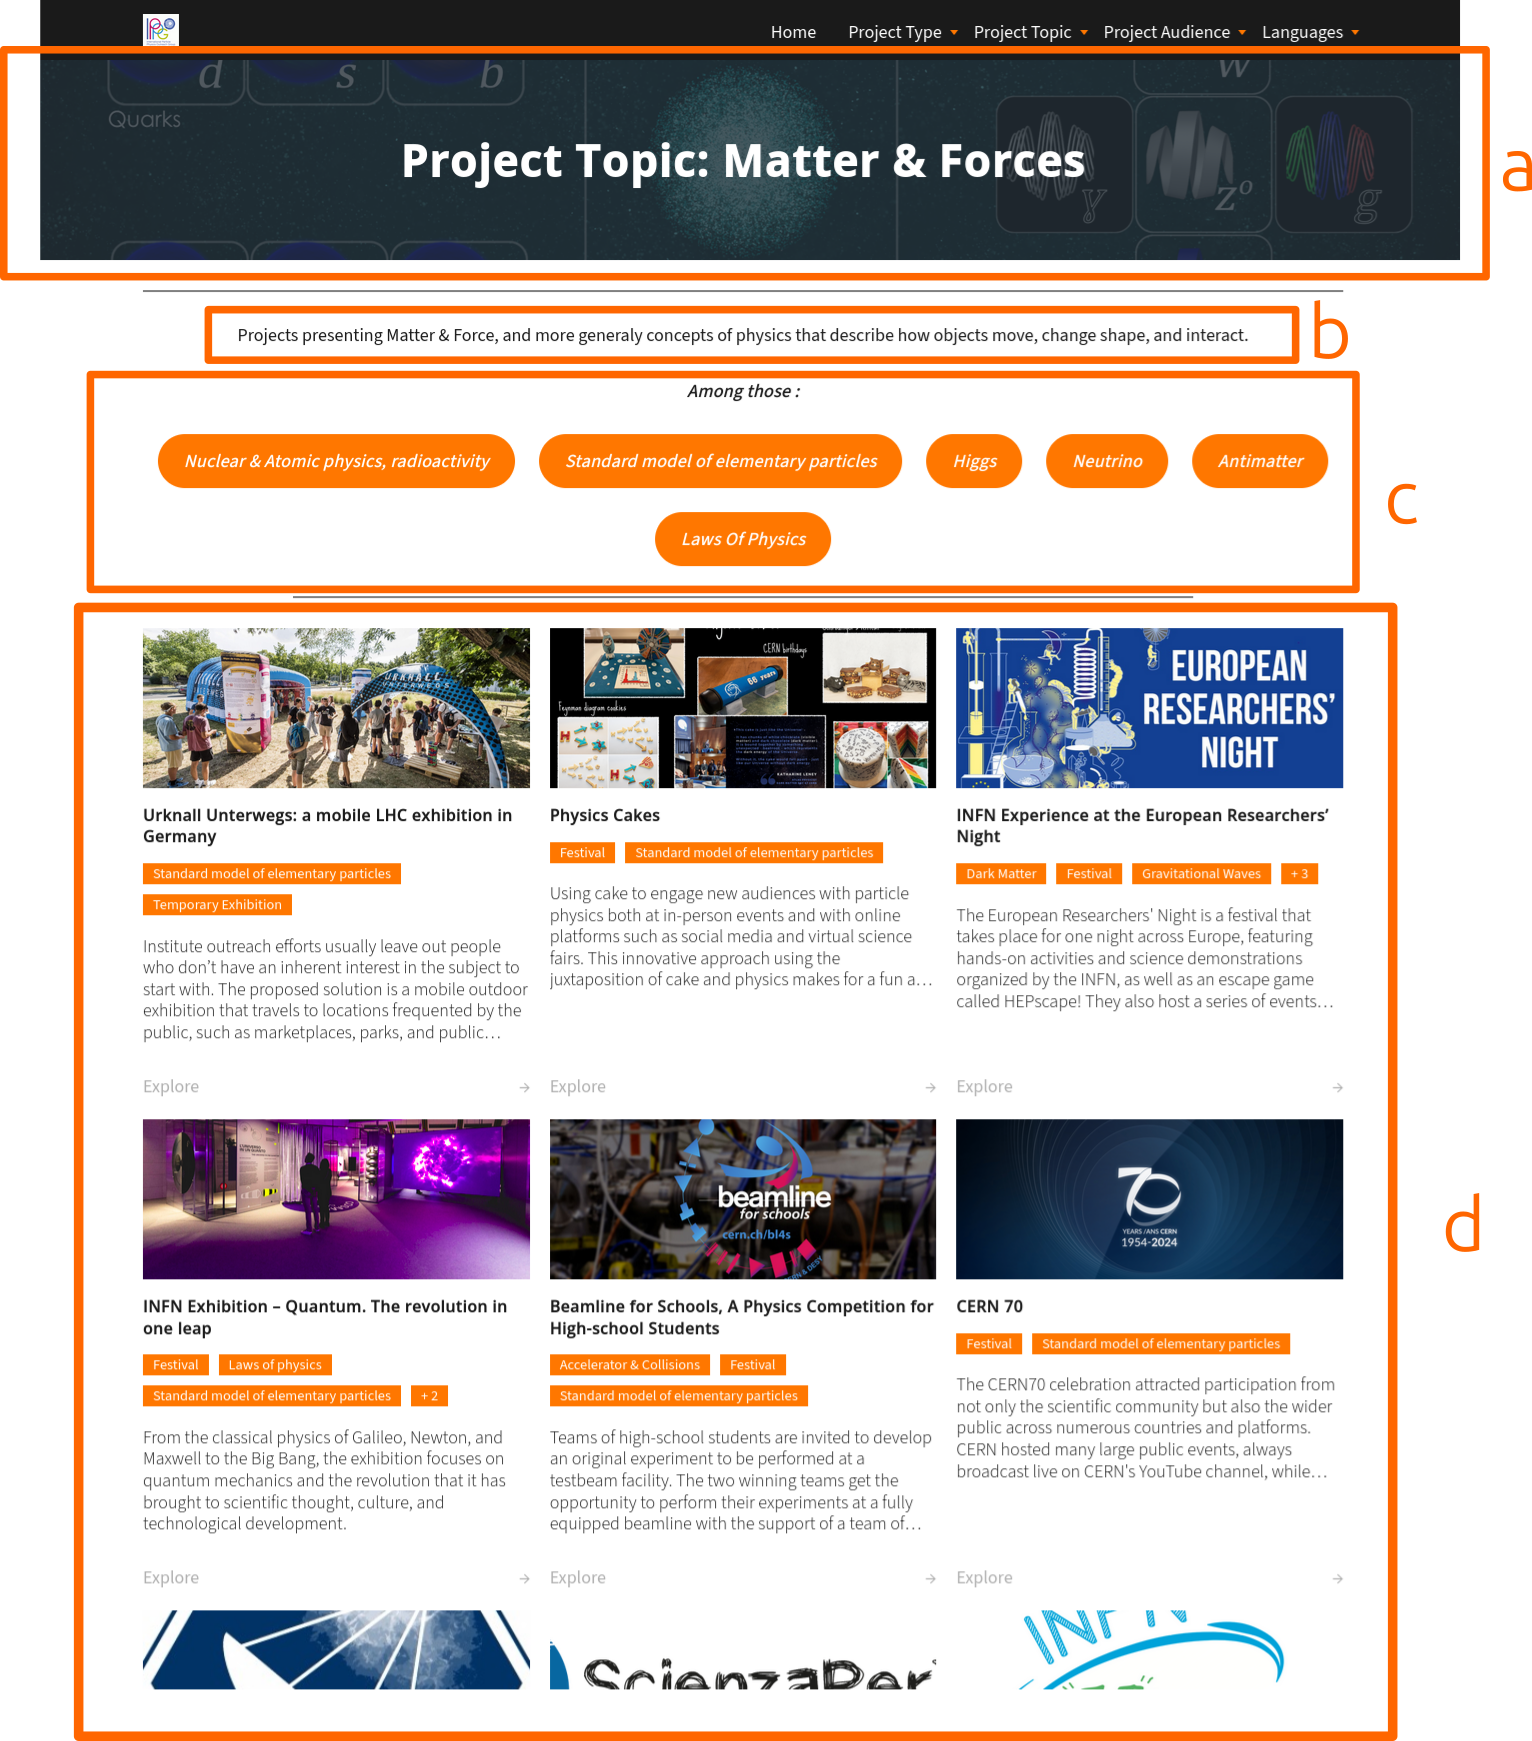
\includegraphics[width=\linewidth]{Image/Architecture/structure_category.png}
    \caption{Categories pages (example of the "Matter \& Forces" page)}
    \label{fig:structure_category}
\end{figure}
\newpage

\section{Languages Categories pages}\label{sec:structure_language}

The language categories (Fig. \ref{fig:structure_language}) are a bit different from other categories. As it aims to form discussion groups, these pages have a strong focus on the countries. Also, all these pages are translated into their own language.

\subsection*{a. Title}
[H1 Title block] with the name of the relative language.

\subsection*{b. Introduction}
[Paragraph block] introducing the members of the collaboration related to the language.

\subsection*{c. IPPOG members}
[Paragraph block] followed by a [List block] listing the representatives of the member countries with a link leading to the IPPOG general website.

\subsection*{d. Countries participating in Masterclass}
[Paragraph block] followed by a [List block] listing the countries (members of IPPOG or not) participating in International Physics Masterclass.

\subsection*{e. Projects}
[News block] displaying all projects with the related language.

\begin{figure}[p]
    \centering
    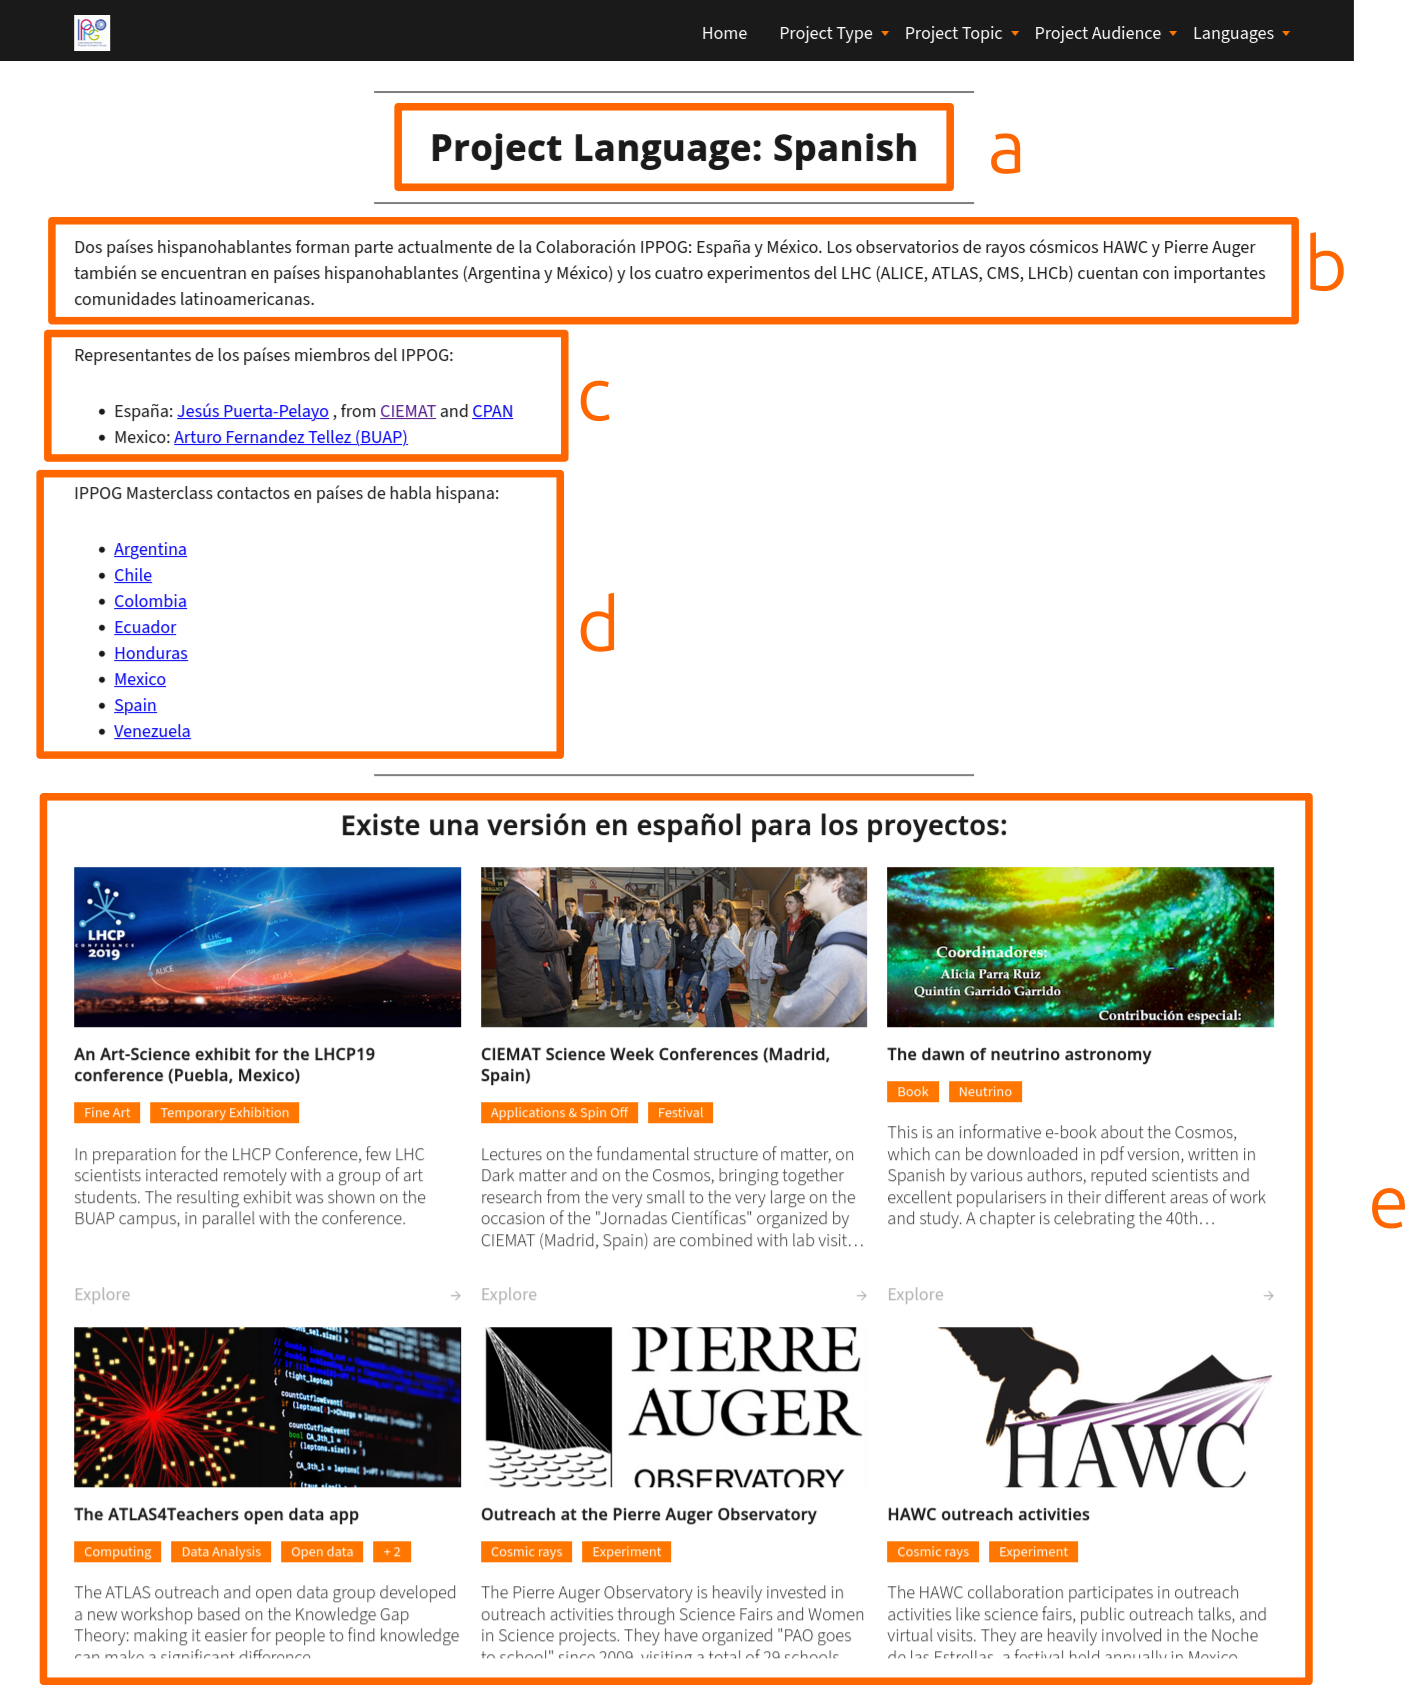
\includegraphics[width=\linewidth]{Image/Architecture/structure_language.png}
    \caption{Language category pages (example of the "Spanish" page)}
    \label{fig:structure_language}
\end{figure}
\newpage

\section{Projects Posts}\label{sec:structure_post}

The Posts (Fig. \ref{fig:structure_post}) present all information relevant to one project. All data are extracted from the database.

\subsection*{a. Title \& Image}
[Media \& Text block] made of the [Featured Image block] of the post on the right, and the [H1 Title block] of the post on the left. There can also be a [H2 Title block] working as a subtitle below the title.

\subsection*{b. Credit for the image}
[Paragraph block] crediting the author of the featured image, aligned on the right.

\subsection*{c. Abstract}
[H2 Title block] "Abstract" followed by a [Paragraph block] briefly describing the project.

\subsection*{d. Presentation slides}
[List block] linking to the presentation of the project during a conference or a meeting.

\subsection*{e. Authors}
[H2 Title block] "Contact" followed by a [Paragraph block] "Authors: " and a [List block] listing the authors of the project and their affiliations.

\subsection*{f. Related IPPOG members}
[Paragraph block] "Related IPPOG Collaboration members:" followed by a [List block] listing the IPPOG members relevant for the project, and linking to the general IPPOG website.

\subsection*{g. Public Contact}
[Paragraph block] "Contact:" followed by a [List block] with either an email or a link to a contact form to contact the authors of the project.

\subsection*{h. Status}
[H2 Title block] "Project status" followed by a [Paragraph block] describing the status of the project and the last time the post was updated.

\subsection*{i. Files \& Resources}
[H2 Title block] "Files \& Resources" followed by a [List block] linking to relevant resources.

\subsection*{j. Categories \& Tags}
[Categories block] and [Tags block] of the post linking to the automatically generated pages (Sec. \ref{sec:structure_auto}).

\begin{figure}[p]
    \centering
    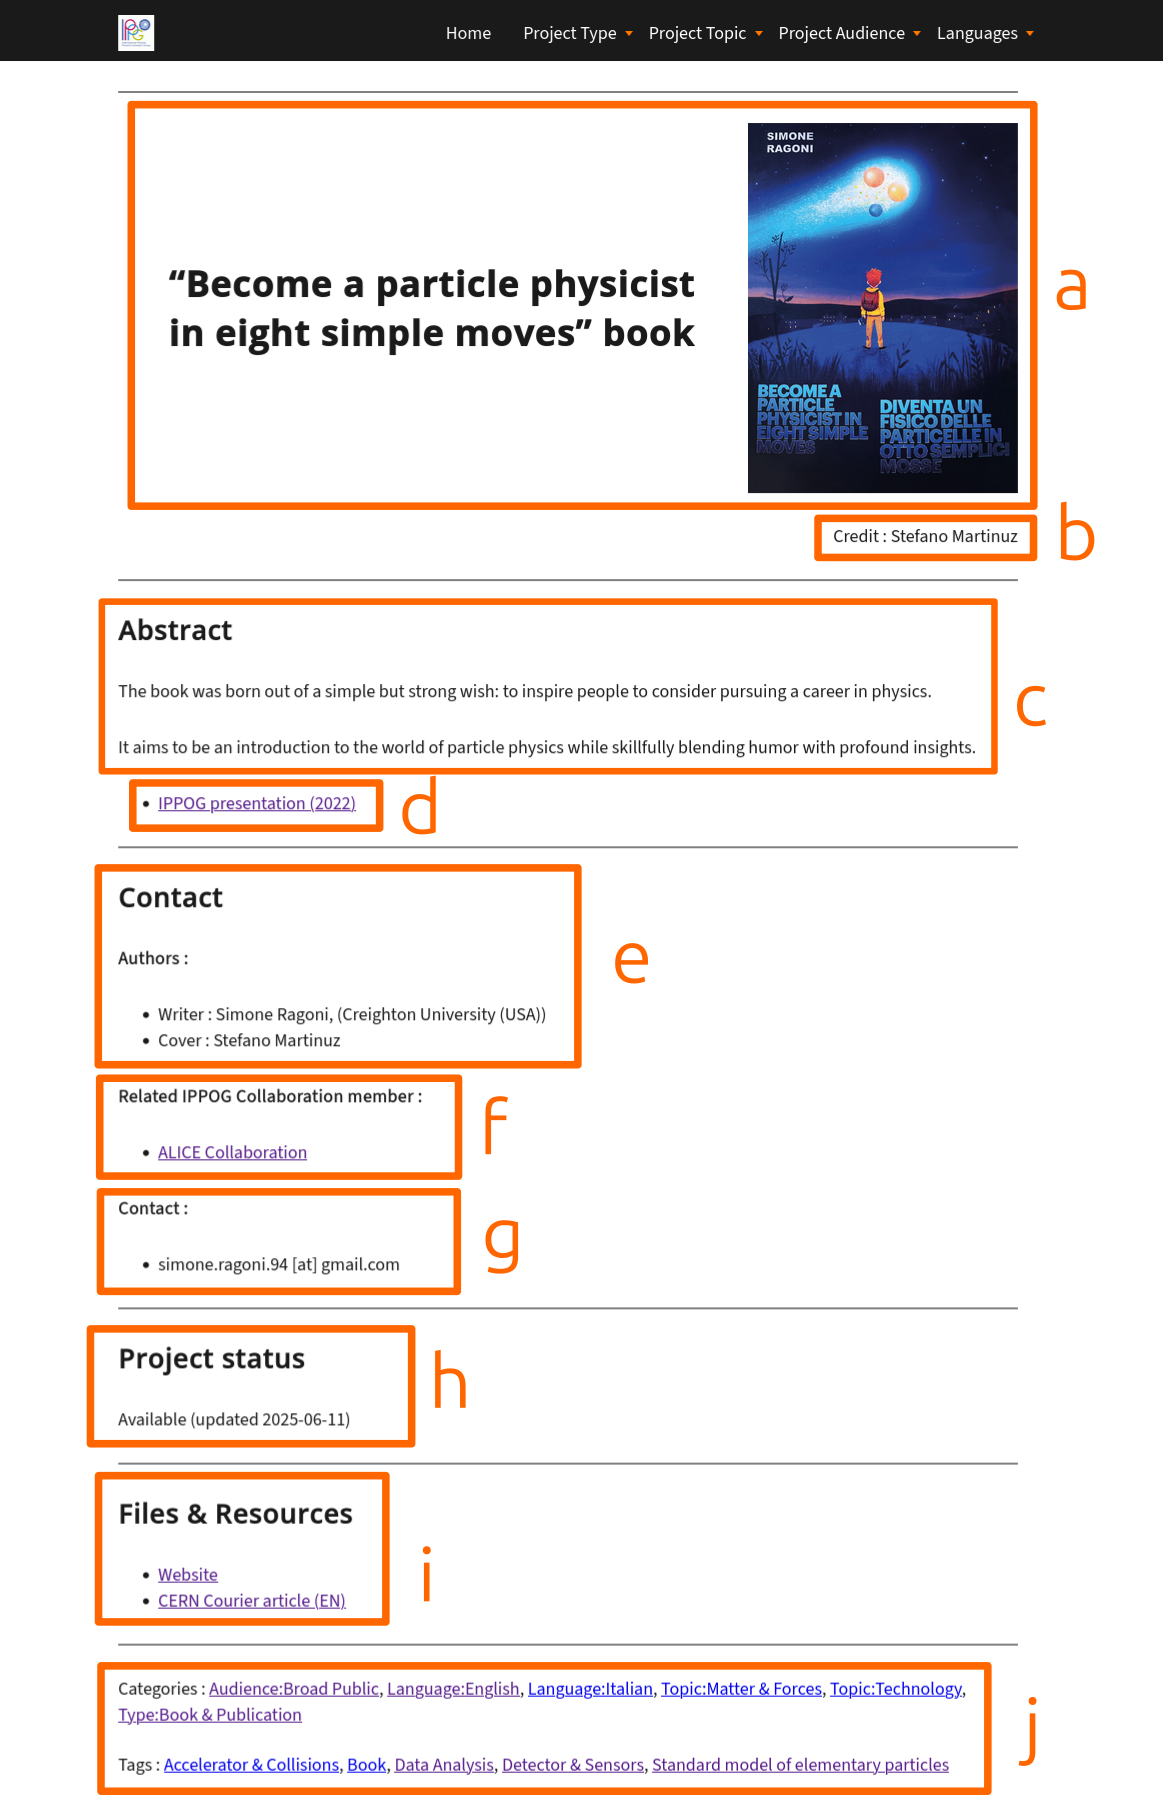
\includegraphics[width=.85\linewidth]{Image/Architecture/structure_project.png}
    \caption{Post pages (example of the “Become a particle physicist in eight simple moves book" post)}
    \label{fig:structure_post}
\end{figure}
\newpage

\section{Categories \& Tags automatic pages}\label{sec:structure_auto}

The WordPress automatically generates pages for each category and tag (Fig. \ref{fig:structure_auto}). Those pages can be accessed either through: 
\begin{itemize}
    \item the links in [News Blocks] (Fig. \ref{fig:structure_auto3}),
    \item at the top of category-specific pages (Fig. \ref{fig:structure_auto2}), or
    \item at the end of posts (Fig. \ref{fig:structure_auto1}).
\end{itemize}   
As they are generated automatically, they cannot be modified at the moment and, as such, they remain not very visually attractive. This is why the choice was made to create easier-to-navigate pages (Sec. \ref{fig:structure_category}).

\bigskip

\begin{figure}[th]
    \begin{subfigure}[c]{.5\textwidth}
        \centering
        \begin{subfigure}[t]{\textwidth}
            \centering
            
\includegraphics[width=\textwidth]{Image/Architecture/structure_auto1.png}
            \caption{at the end of posts}
            \label{fig:structure_auto1}
        \end{subfigure}
        
             
        \vspace{2cm}
        \begin{subfigure}[c]{\textwidth}
            \centering
            
\includegraphics[width=\textwidth]{Image/Architecture/structure_auto2.png}
            \caption{at the top of category-specific pages}
            \label{fig:structure_auto2}
        \end{subfigure}
    \end{subfigure}
    \hfill  % NOTE1: hfill moves horizontally stacked objects as far apart as it can
    \begin{subfigure}[c]{.4\textwidth}
        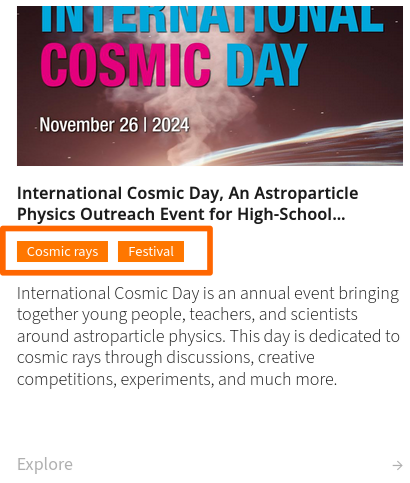
\includegraphics[width=\textwidth]{Image/Architecture/structure_auto3.png}
        \caption{in [News Blocks]}
        \label{fig:structure_auto3}
    \end{subfigure}
    \caption{Links to Categories \& Tags automatic pages}
\end{figure}

\begin{figure}[p]
    \centering
    
\includegraphics[width=\linewidth]{Image/Architecture/structure_auto.png}
    \caption{Categories \& Tags automatic pages}
    \label{fig:structure_auto}
\end{figure}

\newpage

\section{General Information}\label{sec:structure_genaralinfo}

The General Information menu (Fig. \ref{fig:structure_general_info}) links to two pages: a general description of the IPPOG Collaboration (Sec. \ref{ssec:structure_FAQ}) and the Taxonomy used in the website (Sec. \ref{ssec:structure_Categorization})

\smallskip

\begin{figure}[h!]
    \centering
    
\includegraphics[width=.9\linewidth]{Image/Architecture/structure_general_info.png}
    \caption{General Information menu}
    \label{fig:structure_general_info}
\end{figure}

\subsection{FAQ}\label{ssec:structure_FAQ}

The FAQ page (Fig. \ref{fig:structure_faq}) gives a general description of the collaboration.

\subsubsection*{a. Presentation of the IPPOG}
This section presents the IPPOG collaboration, its goals, members, and a few relevant links.

\subsubsection*{b. Flagship activities of the IPPOG}
This section lists the current activities of the IPPOG collaboration.

\subsubsection*{c. Presentation of the Resource Portal}
This is a small presentation of the Resource Portal and why it was created.

\subsubsection*{d. Contact}
Link to the contact form.

\subsection{Categorization}\label{ssec:structure_Categorization}

This page (Fig. \ref{fig:structure_taxonomy}) gives a quick overview of the taxonomy used to classify the projects on the website.

\subsubsection*{a. Introduction}
This section gives a small introduction to the taxonomy.

\subsubsection*{b. Taxonomy}
This is the infographic available in Fig \ref{fig:Topics_category} \& \ref{fig:Types_category}. These are created using the FraMindmap software (Sec. \ref{sec:map}).

\begin{landscape}
    
    \begin{figure}[p]
        \centering
        \begin{subfigure}[c]{.5\textwidth}
            \centering
            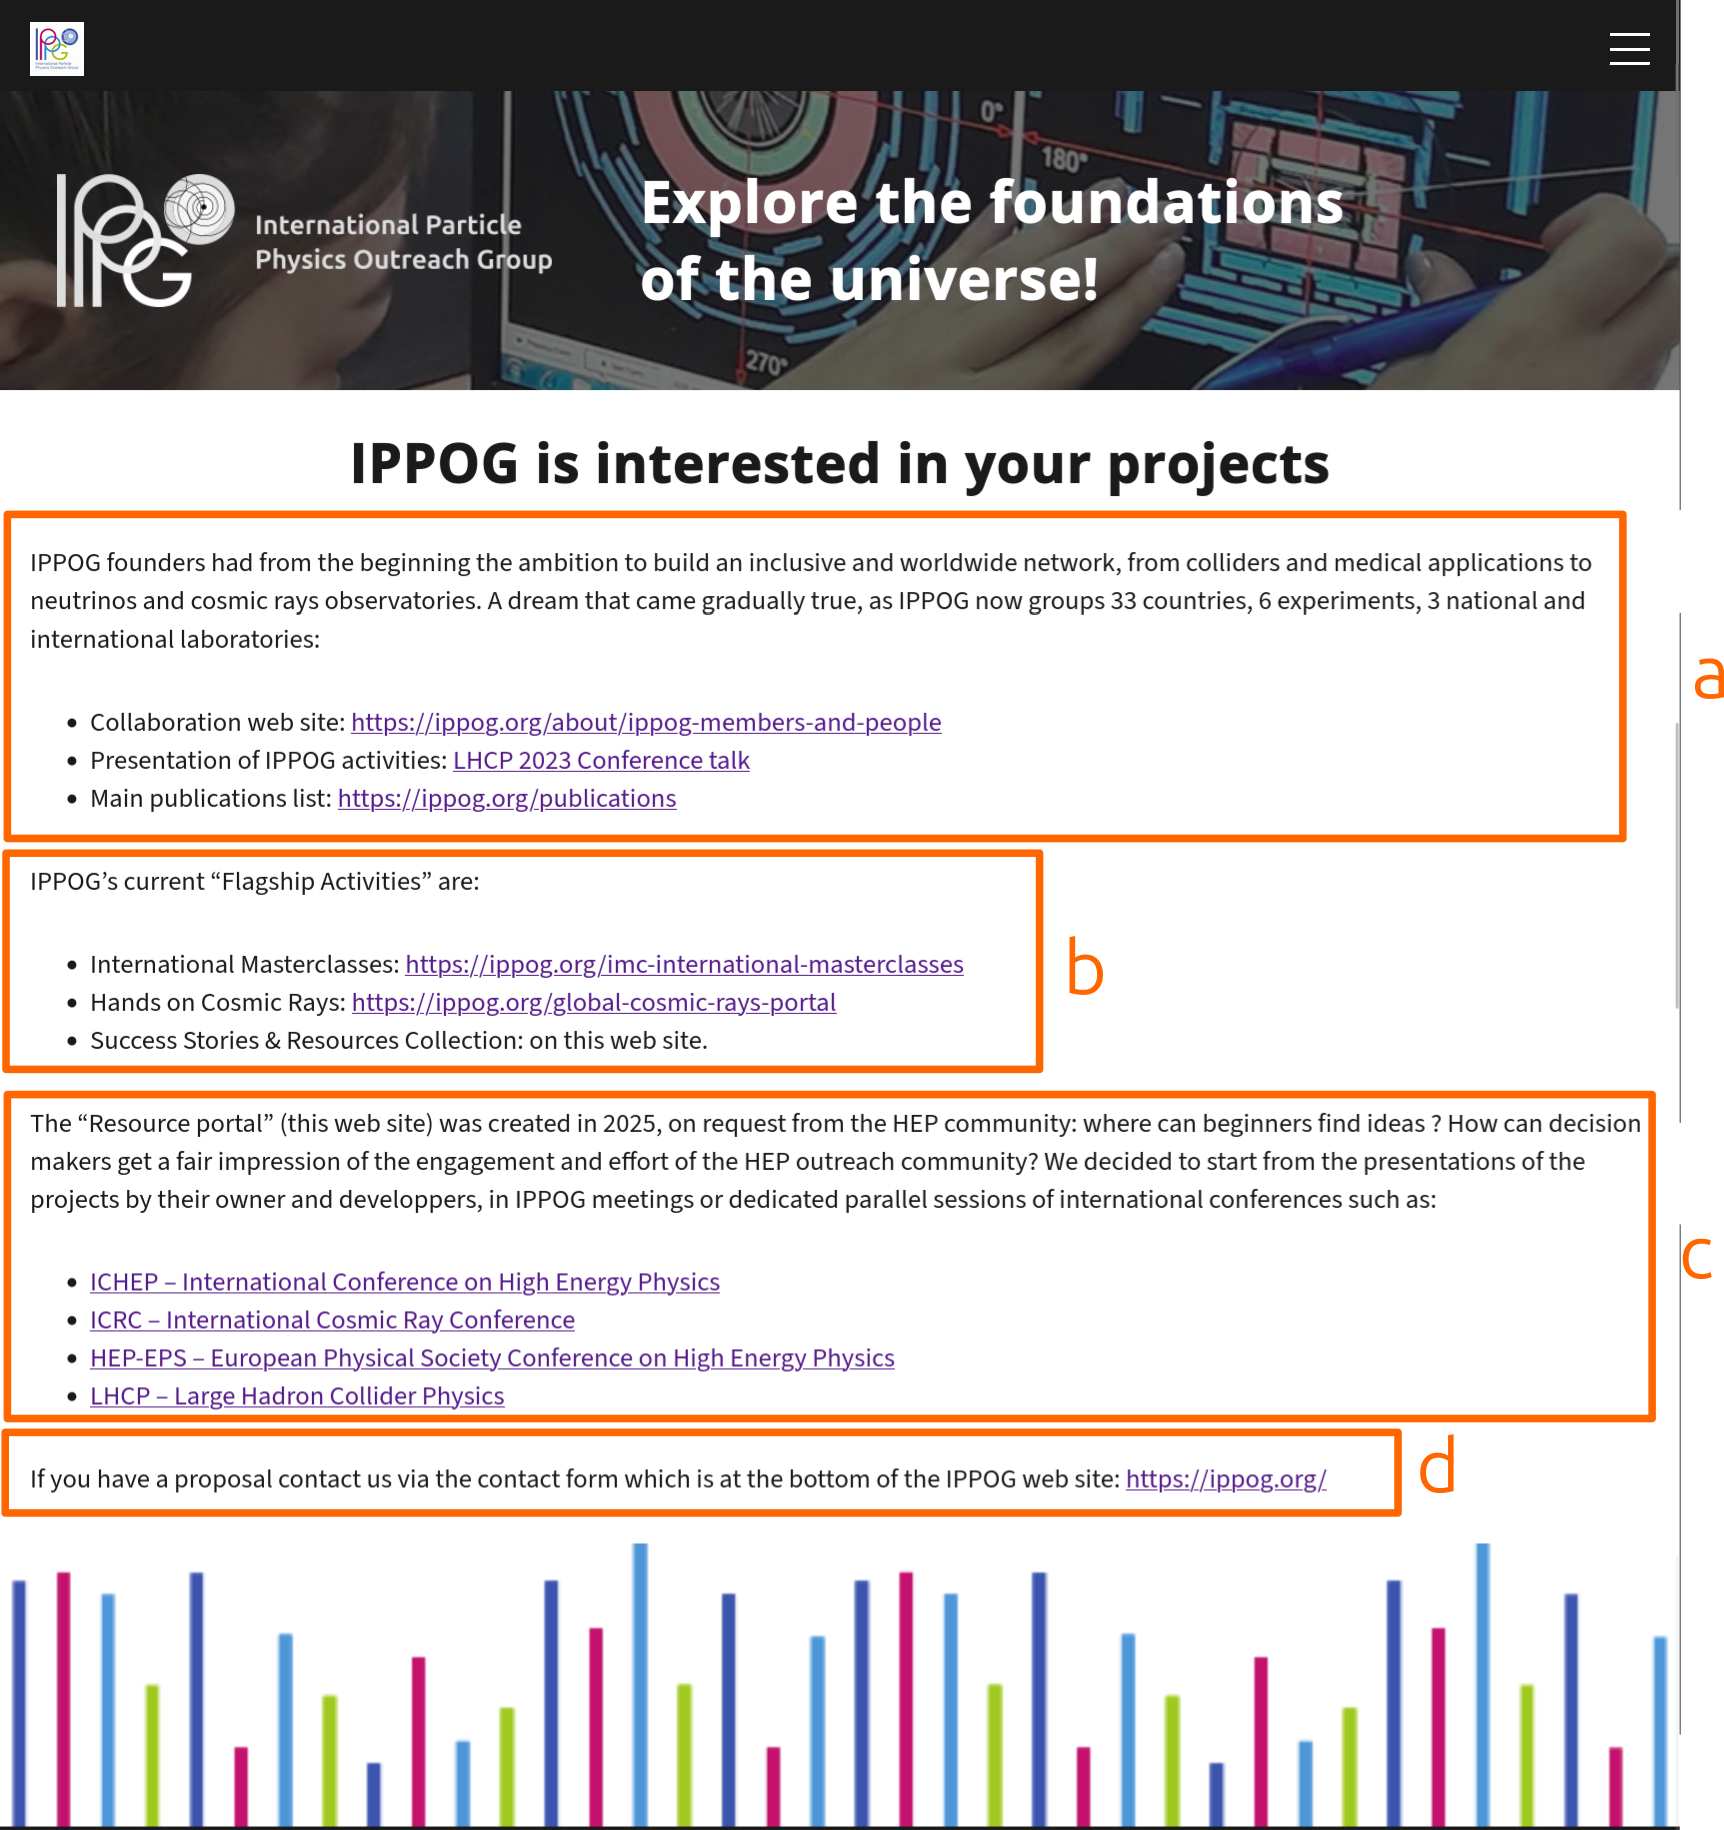
\includegraphics[width=1.2\linewidth]{Image/Architecture/structure_faq.png}
            \caption{FAQ page}
            \label{fig:structure_faq}
        \end{subfigure}
        \hspace{3cm}
        \begin{subfigure}[c]{.5\textwidth}
            \centering
            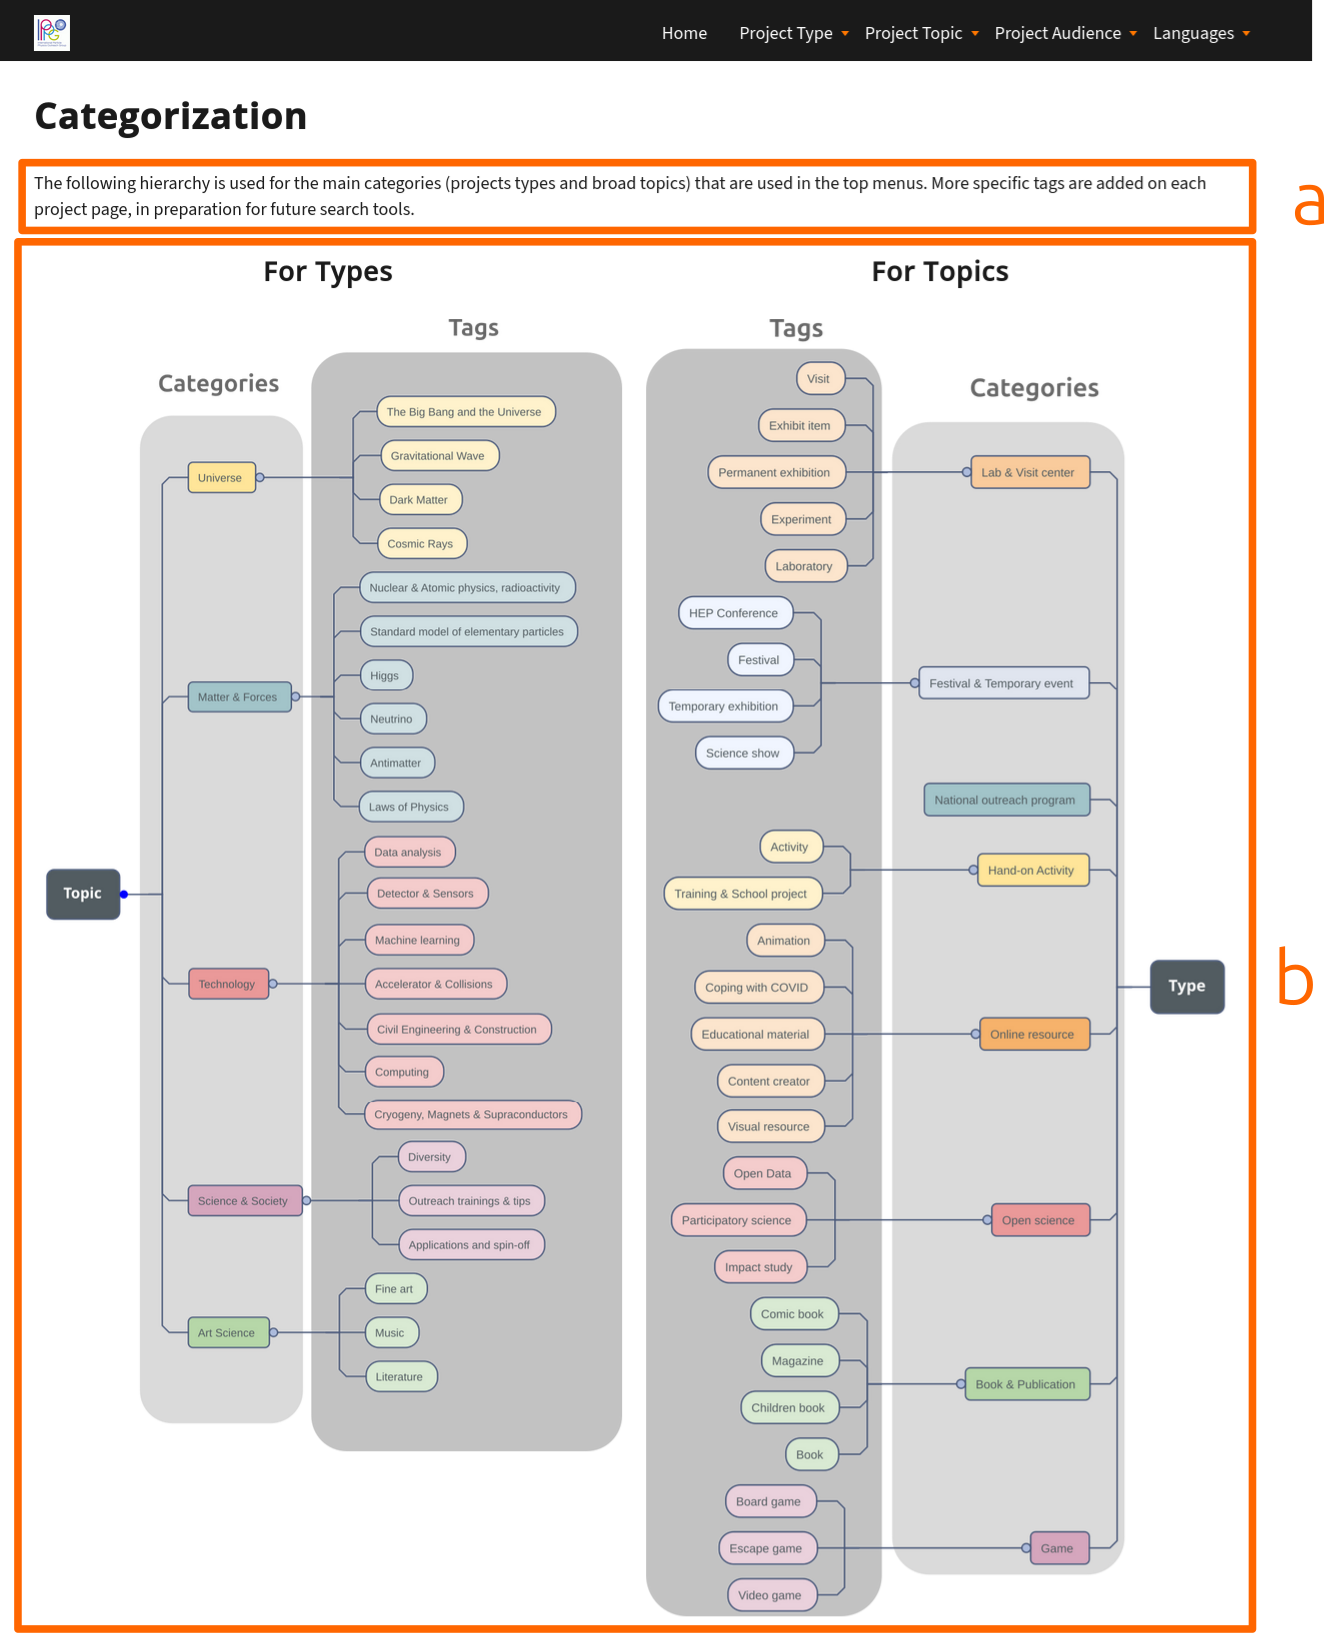
\includegraphics[width=1.2\linewidth]{Image/Architecture/structure_taxonomy.png}
            \caption{Taxonomy page}
            \label{fig:structure_taxonomy}
        \end{subfigure}
        \label{fig:gform}
        \caption{General Information menu}
    \end{figure}

\end{landscape}
\chapter{Upload Process}\label{chap:process}

This chapter explains the whole process of uploading Posts on the website, from filling out the Google form (Section \ref{sec:googleform}) linked to a database on Google Sheet (Section \ref{sec:googlesheet}), to running the Python code (Section \ref{sec:Python}) that formats the data into text that can be copy-pasted on the website (Section \ref{sec:upload}). A flowchart summarizing the process is available below (Fig \ref{fig:flowchart}).

\begin{landscape}
    %\documentclass{standalone}
%\usepackage{tikz}
%\def\checkmark{\tikz\fill[scale=0.4](0,.35) -- (.25,0) -- (1,.7) -- (.25,.15) -- cycle;} 
%\usetikzlibrary{arrows,shapes,positioning,shadows,trees}
%\usetikzlibrary{decorations.markings}

%\begin{document}

\tikzstyle{startstop} = [rectangle, rounded corners, 
minimum width=3cm, 
minimum height=1cm,
text centered, 
draw=black, 
fill=red!30]

\tikzstyle{io} = [trapezium, 
trapezium stretches=true, % A later addition
trapezium left angle=70, 
trapezium right angle=110, 
text width=3cm, 
minimum width=3cm, 
minimum height=1cm, text centered, 
draw=black, fill=blue!30]

\tikzstyle{process} = [rectangle, 
minimum width=3cm, 
minimum height=1cm, 
text centered, 
text width=3cm, 
draw=black, 
fill=orange!30]

\tikzstyle{decision} = [diamond, 
minimum width=.5cm, 
aspect=2,
minimum height=.5cm,  
text width=2cm, 
text centered, 
draw=black, 
fill=green!30]
\tikzstyle{arrow} = [thick,->,>=stealth]

\begin{figure}[h!]
    \centering
    \begin{tikzpicture}[node distance=2cm]
        \vspace{1cm}
        
        \node (inform) [io] {Input (User/IPPOG)};
        \node (form) [startstop, below of=inform, yshift=-.5cm] {Google form};
        
        \node (online) [process, below of=form, yshift=-.5cm] {Google sheet database};
        \node (inonline) [io, below of=online, yshift=-.5cm] {Correction (IPPOG)};
        
        \node (decision) [decision, right of=online, xshift=2.5cm] {Choice};
        
        \node (inlocal) [io, above of=decision, yshift=.5cm] {Download CSV File (IPPOG)};
        \node (local) [process, right of=inlocal, xshift=2.5cm] {Local CSV file database};
        
        \node (inpylocal) [io, right of=local, xshift=2.5cm] {run\_local.py (IPPOG)};
        \node (pylocal) [process, right of=inpylocal, xshift=2.5cm] {Python local code};
        \node (inpyonline) [io, below of=inpylocal, yshift=-.5cm] {run\_online.py (IPPOG)};
        \node (pyonline) [process, right of=inpyonline, xshift=2.5cm] {Python online code};
        
        \node (md) [process, below of=pyonline, xshift=2.5cm, yshift=-.5cm] {Markdown files};
        
        \node (inmd) [io, below of=md, yshift=-.5cm, xshift=-2.5cm] {Copy/Past (IPPOG)};
        
        \node (web) [startstop, left of=inmd, xshift=-3cm] {Upload to Website};

        \begin{scope}[very thick,decoration={
            markings,
            mark=at position 0.7 with {\arrow{latex}}}
            ] 
            \draw [postaction={decorate}] (0,2) -- (inform);
            \draw [postaction={decorate}] (form) -- node [left] {Auto} (online);
            \draw [postaction={decorate}] (inform) -- (form);
            \draw [postaction={decorate}] (inonline) -- node [right] {Add tags and change status to "OK"}  (online);
            \draw [postaction={decorate}] (online) -- (decision);
            \draw [postaction={decorate}] (decision) -- node [above] {"online" mode} (inpyonline);
            \draw [postaction={decorate}] (decision) -- node [right] {"local" mode} (inlocal);
            \draw [postaction={decorate}] (inlocal) -- (local);
            \draw [postaction={decorate}] (local) -- (inpylocal);
            \draw [postaction={decorate}] (inpylocal) -- (pylocal);
            \draw [postaction={decorate}] (inpyonline) -- (pyonline);
            \draw [postaction={decorate}] (pylocal) -| +(2.5,-2.5);
            %\draw [postaction={decorate}] (pyonline) -+ (21.5,0);
            \draw [postaction={decorate}] (pyonline) -| (md);
            \draw [postaction={decorate}] (pyonline) -- +(2.5,0);
            %\draw [postaction={decorate}] (pylocal) -| (md);
            \draw [postaction={decorate}] (md) |- (inmd);
            \draw [postaction={decorate}] (inmd) -- (web);
            \draw [dotted,postaction={decorate}] (md) -- node [below] {Possible to do correction but need to be recompiled} (inonline);
            \draw [dotted,postaction={decorate}] (web) -- node [below] {Change status to "Online"} (-2.5,-10);
            \draw [dotted,postaction={decorate}] (-2.5,-10) |- (online);
        \end{scope}
    \end{tikzpicture}
    \caption{Flowchart of the upload process}
    \label{fig:flowchart}
\end{figure}


%\end{document}%\label{fig:flowchart}
\end{landscape}

\section{Submitting projects through the Google form}\label{sec:googleform}

To facilitate the filling of the database, it was decided to use the option of linking a Google form to a Google Sheet document. It allows to guide the user through the form (Fig. \ref{fig:gform}), and to automatically fill the database on Google Sheet.

All fields of the form are detailed in Table \ref{tab:form_description}, with a description and whether the field is mandatory or not. It is important that the user follows the explicit format, in the case of the authors: "Author1,Afficiation1\textbackslash n". Otherwise the Python code formatting the database will not understand and will not recognize it. 

\begin{figure}[h!]
    \centering
    \begin{subfigure}[c]{.6\textwidth}
        \centering
        
\includegraphics[width=\linewidth]{Image/Process/gform.png}
    \end{subfigure}
    \bigskip
    \begin{subfigure}[c]{.6\textwidth}
        \centering
        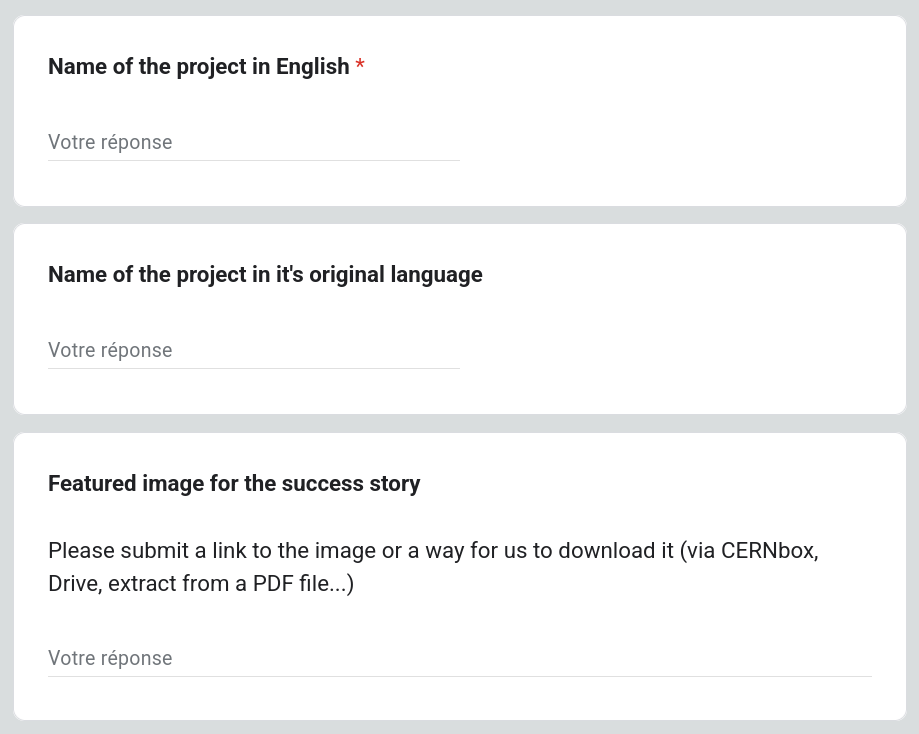
\includegraphics[width=\linewidth]{Image/Process/gform2.png}
    \end{subfigure}
    \caption{Google form interface}
    \label{fig:gform}
\end{figure}

\begin{landscape}
    \begin{table}[]
        \begin{tabularx}{\linewidth}{|lc|X|}
            \hline
            \multicolumn{1}{|l|}{\textbf{Name}} & \textbf{\begin{tabular}[c]{@{}l@{}}Mandatory\\\end{tabular}} & \textbf{Description} \\ \hline
            \multicolumn{2}{|c|}{\textbf{Main}} &  \\ \hline
            \rowcolor[HTML]{EFEFEF}
            \multicolumn{1}{|l|}{Name of the project in English} & \checkmark &  \\ \hline
            \multicolumn{1}{|l|}{Name of the project in its original language} & &  \\ \hline
            \multicolumn{1}{|l|}{Featured image for the success story} & & Link to the image or a way for us to download it \\ \hline
            \multicolumn{1}{|l|}{Credit of the featured image} & &  \\ \hline
            \rowcolor[HTML]{EFEFEF}
            \multicolumn{1}{|l|}{Abstract of the Project} & \checkmark & Abstract should be about 500 characters \\ \hline
            \multicolumn{2}{|c|}{\textbf{Contact}} &  \\ \hline
            \rowcolor[HTML]{EFEFEF}
            \multicolumn{1}{|l|}{Authors of the project and affiliations} & \checkmark & \begin{tabular}[c]{@{}l@{}}The input should take the form: \\ Author1,Afficiation1\\ Author2,Affiliation2\\ ...\\ With one author per line with no space, otherwise it will not be\\recognized by the python code\end{tabular} \\ \hline
            \rowcolor[HTML]{EFEFEF}
            \multicolumn{1}{|l|}{Public contact} & \checkmark & If an email is given, the @ sign should be replaced by "{[} at {]}" on the website (this is done automatically by the python program) \\ \hline
            \multicolumn{1}{|l|}{Private contact for the core team} & & This should not appear on the website, only in the private database \\ \hline
            \rowcolor[HTML]{EFEFEF}
            \multicolumn{1}{|l|}{Status of the project} & \checkmark & multiple choice \\ \hline
            \multicolumn{2}{|c|}{\textbf{Presented conference / meeting}} &  \\ \hline
            \multicolumn{1}{|l|}{Name of the conference / meeting} & &  \\ \hline
            \multicolumn{1}{|l|}{Year of the conference / meeting} & &  \\ \hline
            \multicolumn{1}{|l|}{URL to the presentation slides / publication} & &  \\ \hline
            \multicolumn{2}{|c|}{\textbf{Related resources}} &  \\ \hline
            \multicolumn{1}{|l|}{Other project resources} & & \begin{tabular}[c]{@{}l@{}}The input should take the form: \\ ResourceName1(Language):URL1\\ ResourceName2(Language):URL2\\ ...\\ With one resource per line with no space, otherwise it will not be\\recognizedby the python code\end{tabular} \\ \hline
            \multicolumn{2}{|c|}{\textbf{Categories}} & check box \\ \hline
            \rowcolor[HTML]{EFEFEF}
            \multicolumn{1}{|l|}{Type of the project} & \checkmark & check box \\ \hline
            \rowcolor[HTML]{EFEFEF}
            \multicolumn{1}{|l|}{Topic of the project} & \checkmark & check box \\ \hline
            \rowcolor[HTML]{EFEFEF}
            \multicolumn{1}{|l|}{Audiences} & \checkmark & check box \\ \hline
            \multicolumn{1}{|l|}{Languages of the project} & &  \\ \hline
            \multicolumn{1}{|l|}{Related IPPOG countries, experiments or laboratories} & & check box \\ \hline
        \end{tabularx}
        \caption{Description of the Google form fields}
        \label{tab:form_description}
    \end{table}
\end{landscape}

\section{Registering the projects in the Google Sheet database}\label{sec:googlesheet}

The choice of using a database was to be able to easily archive it in CERNbox or other cloud, in case of data loss, but also to enable the scientific community to submit their projects that can then be validated or completed by the core team or the person responsible for the resource portal.

The database is composed of 5 pages
\begin{itemize}
    \item \textit{Réponse au formulaire 1}: The raw submitted data from the Google Form appears here.
    \item \textit{Work in progress}: Is a transit page where the raw data can be modified without touching the \textit{Full database}.
    \item \textit{Full database}: Is the actual data (Table \ref{tab:database_description}). Few columns need to be modified manually by the user: 
    \begin{itemize}
        \item First, the user should clear the content of the first column "Horodateur" from \textit{Réponse au formulaire 1} and copy and paste the data to a new empty line.
        \item Column A "ID" should be given an unused ID.
        \item Columns B to T should already be filled.
        \item Column U "Sub Type" and V "Sub Topics" should be given related tags according to the taxonomy (Sec. \ref{ssec:categorization}).
        \item Column W "Wordpress page" should automatically update with the ID from column A, if not the user can copy the formula from the cell above.
        \item Column X "State" should be updated by the used according to the state of the Wordpress page (note that the state should be "OK" for the line to be read by the python code (Section \ref{sec:Python}).
    \end{itemize}
    \item \textit{Proposition}: Is a list of projects that were either rejected or put aside for later.
    \item \textit{Copy of Full database}: Is a copy of the \textit{Full database} page.
\end{itemize}

The database is then read by a python code (Section \ref{sec:Python}) that produce one formatted markdown file per project.

\begin{landscape}
    \begin{table}[]
        \begin{tabularx}{\linewidth}{|cXcc|X|}
            \hline
            \multicolumn{1}{|l|}{\textbf{Column}} & \multicolumn{1}{l|}{\textbf{Name}} & \multicolumn{1}{l|}{\textbf{Google Form}} & \textbf{Manually} & \textbf{Description} \\ \hline
            \multicolumn{1}{|c|}{A} & \multicolumn{1}{l|}{ID} & \multicolumn{1}{c|}{} & \checkmark & Needs to be manually added according to the previous project ID \\ \hline
            \multicolumn{4}{|c|}{\textbf{Main}} &  \\ \hline
            \multicolumn{1}{|c|}{B} & \multicolumn{1}{l|}{Name of the project in English} & \multicolumn{1}{c|}{\checkmark} &  &  \\ \hline
            \multicolumn{1}{|c|}{C} & \multicolumn{1}{l|}{Name of the project in its original language} & \multicolumn{1}{c|}{\checkmark} &  &  \\ \hline
            \multicolumn{1}{|c|}{D} & \multicolumn{1}{l|}{Featured Image} & \multicolumn{1}{c|}{} & \checkmark & User gives a means to download the image, but the core team needs to upload the image in CERNbox and put the shared link here \\ \hline
            \multicolumn{1}{|c|}{E} & \multicolumn{1}{l|}{Credit of the featured image} & \multicolumn{1}{c|}{\checkmark} &  &  \\ \hline
            \multicolumn{1}{|c|}{F} & \multicolumn{1}{l|}{Abstract} & \multicolumn{1}{c|}{\checkmark} &  &  \\ \hline
            \multicolumn{4}{|c|}{\textbf{Contact}} &  \\ \hline
            \multicolumn{1}{|c|}{G} & \multicolumn{1}{l|}{Author names,affiliation} & \multicolumn{1}{c|}{\checkmark} &  &  \\ \hline
            \multicolumn{1}{|c|}{H} & \multicolumn{1}{l|}{Supporting entities} & \multicolumn{1}{c|}{} & \checkmark & Deprecated but kept in case it would be needed again \\ \hline
            \multicolumn{1}{|c|}{I} & \multicolumn{1}{l|}{Public contact} & \multicolumn{1}{c|}{\checkmark} &  &  \\ \hline
            \multicolumn{1}{|c|}{J} & \multicolumn{1}{l|}{Private contact} & \multicolumn{1}{c|}{\checkmark} &  &  \\ \hline
            \multicolumn{1}{|c|}{K} & \multicolumn{1}{l|}{Project Status} & \multicolumn{1}{c|}{\checkmark} &  &  \\ \hline
            \multicolumn{4}{|c|}{\textbf{Presented conference / meeting}} &  \\ \hline
            \multicolumn{1}{|c|}{L} & \multicolumn{1}{l|}{Name of the conference} & \multicolumn{1}{c|}{\checkmark} &  &  \\ \hline
            \multicolumn{1}{|c|}{M} & \multicolumn{1}{l|}{Year of the conference} & \multicolumn{1}{c|}{\checkmark} &  &  \\ \hline
            \multicolumn{1}{|c|}{N} & \multicolumn{1}{l|}{Presentation Documents} & \multicolumn{1}{c|}{\checkmark} &  &  \\ \hline
            \multicolumn{4}{|c|}{\textbf{Related resources}} &  \\ \hline
            \multicolumn{1}{|c|}{O} & \multicolumn{1}{l|}{Other resources} & \multicolumn{1}{c|}{\checkmark} &  &  \\ \hline
            \multicolumn{4}{|c|}{\textbf{Categories}} &  \\ \hline
            \multicolumn{1}{|c|}{P} & \multicolumn{1}{l|}{Type} & \multicolumn{1}{c|}{\checkmark} &  &  \\ \hline
            \multicolumn{1}{|c|}{Q} & \multicolumn{1}{l|}{Topics} & \multicolumn{1}{c|}{\checkmark} &  &  \\ \hline
            \multicolumn{1}{|c|}{R} & \multicolumn{1}{l|}{Audiences} & \multicolumn{1}{c|}{\checkmark} &  &  \\ \hline
            \multicolumn{1}{|c|}{S} & \multicolumn{1}{l|}{Language} & \multicolumn{1}{c|}{\checkmark} &  &  \\ \hline
            \multicolumn{1}{|c|}{T} & \multicolumn{1}{l|}{Related IPPOG member} & \multicolumn{1}{c|}{\checkmark} &  &  \\ \hline
            \multicolumn{1}{|c|}{U} & \multicolumn{1}{l|}{Sub Types} & \multicolumn{1}{c|}{} & \checkmark & Should be completed using the types map \\ \hline
            \multicolumn{1}{|c|}{V} & \multicolumn{1}{l|}{Sub Topics} & \multicolumn{1}{c|}{} & \checkmark & Should be completed using the topics map \\ \hline
            \multicolumn{4}{|c|}{\textbf{Private}} &  \\ \hline
            \multicolumn{1}{|c|}{W} & \multicolumn{1}{l|}{Wordpress page} & \multicolumn{1}{c|}{} & \checkmark & URL to the wordpress page: https://ippog-resources-portal.web.cern.ch/project-\{Column A\} \\ \hline
            \multicolumn{1}{|c|}{X} & \multicolumn{1}{l|}{State} & \multicolumn{1}{c|}{} & \checkmark & Should be updated depending (see above) \\ \hline
        \end{tabularx}
        \caption{Description of the database per columns}
        \label{tab:database_description}
    \end{table}
\end{landscape}

\section{Formatting the projects with a Python code}\label{sec:Python}

The code is available in github: 
\begin{lstlisting}[language=Python]
    git clone https://github.com/Troy314/IPPOG_Website.git
\end{lstlisting}

\begin{itemize}
    \item \gray{dictionaries/member\_dictionary.py} is a dictionary which take the entry from Column T "Related IPPOG member" and return the url to the corresponding page in the IPPOG website\footnote{Members and people of the IPPOG Collaboration: \href{https://ippog.org/about/ippog-members-and-people}{https://ippog.org/about/ippog-members-and-people}}
    \item \gray{run\_local.py} \& \gray{run\_online.py} files are the codes that create the markdown files
    \item \gray{output\_markdown/} is the filder in which markdowns are created
    \item \gray{exemple\_file.csv} is a document that has the format of the database and can be used to test the run codes 
\end{itemize}

\subsection{Dependencies}\label{dependencies}

Libraries needed to run the code are: 

\begin{lstlisting}[language=Python]
    python3 -m pip install python-csv DateTime pathlib2
\end{lstlisting}

Optional parts of the code makes use of Google Sheets API and needs:

\begin{lstlisting}[language=Python]
    python3 -m pip install gspread google-auth google-auth-oauthlib google-auth-httplib2
\end{lstlisting}

\subsection{Running}

Two version of the code are available
\begin{itemize}
    \item \gray{run\_local.py}: directly extract data through Google's API (need the optional dependencies)
    \item \gray{run\_online.py}: extract data from a local CSV file 
\end{itemize}

\begin{multicols}{2}
    \raggedcolumns
    \subsubsection*{Online mode}
    
        /!\textbackslash \ Require the use of Google API, see Sec. \ref{ssec:API}.\newline
        /!\textbackslash \ Require optional dependencies, see Sec. \ref{dependencies}\newline
        /!\textbackslash \ The JSON file should be put in the same folder as the run file
        
        To run the program, simply run
        \begin{lstlisting}[language=Python]
        python3 run_online.py\end{lstlisting}
    \columnbreak
    \subsubsection*{Local mode}
    
        /!\textbackslash \ Require to download the database available on Google sheet\footnote{Google Sheet: \href{https://docs.google.com/spreadsheets/d/1x_SdxdlHwG8chH77WqrTAAgijY2XBY3nPIi2p3TKqzs/edit?gid=1297224389\#gid=1297224389}{https://shorturl.at/sHBrz}} as a CSV file\newline
        \vspace{.5cm}
        /!\textbackslash \ The CSV file should be put in the same folder as the run file
    
        To run the program, simply run
        \begin{lstlisting}[language=Python]
        python3 run_local.py\end{lstlisting}
    
        The codes will then ask the name of the CSV file containing the database.
\end{multicols}

Once you run the code, you have two options:
\begin{itemize}
    \item Press [Enter] and run through all projects of which [\textbf{Status = "OK"}] (column X of the database), or
    \item Enter a number, the ID of a project, to force the code to run through a specific project
\end{itemize}

The codes finally produces a \textit{output\_markdown} folder in which each markdown files correspond to a project. The text of each of them should be  copied in a new Post of the website.

\subsection{Enabling Google Sheets API}\label{ssec:API}
This section is about how to use the "online" versions of the code, using the API of Google
/!\textbackslash \ If you are using the "local" version of the code or if you already have the JSON file, you can skip this part

To extract the data from the Google Sheets database, the Google Sheets API needs to be enabled and obtain credentials\footnote{Courtesy to Mayank Gupta: \href{https://dev.to/mayankcse/google-sheets-integration-with-python-a-step-by-step-guide-2mdb}{dev.to/mayankcse/google-sheets-integration-with-python-a-step-by-step-guide-2mdb}}.

\subsubsection*{Enable API Access}

\begin{enumerate}
    \item Go to the Google Cloud Console\footnote{\href{https://console.cloud.google.com/}{Google Cloud Console: https://console.cloud.google.com/}}.
    \item Create a new project (or select an existing one).
    \item Navigate to APIs \& Services > Library.
    \item Search for Google Sheets API and enable it.
    \item Also, enable the Google Drive API (needed for file access permissions).
\end{enumerate}

\subsubsection*{Create Service Account Credentials}

\begin{enumerate}
    \item Go to APIs \& Services > Credentials.
    \item Click on Create Credentials > Service Account.
    \item Assign it a name and click Create \& Continue.
    \item Under "Grant this service account access," select Reading role (optional but useful).
    \item After creating, go to the Keys tab and click Add Key > JSON.
    \item Download the JSON file (keep it secure).
\end{enumerate}

\subsubsection*{Share Your Google Sheet}

\begin{enumerate}
    \item Open the Google Sheet where the database is located.
    \item Click Share and add the email address from the service account JSON file.
    \item Set permissions to Reading.
\end{enumerate}

\section{Uploading the projects on the Website}\label{sec:upload}

The following section will cover how to upload the data generated by the python code on the website. However, it will not explain how to maintain the WordPress infrastructure generally. More information can be found at CERN WordPress Documentation\footnote{CERN WordPress Documentation: \href{https://wordpress.docs.cern.ch/}{https://wordpress.docs.cern.ch/}} and in the dedicated Mattermost channel\footnote{Mattermost channel: \href{https://mattermost.web.cern.ch/it-dep/channels/wordpress}{https://mattermost.web.cern.ch/it-dep/channels/wordpress}}.

A video guide\footnote{Video guide: \href{https://www.youtube.com/watch?v=OQ6QYBG_MYU}{https://www.youtube.com/watch?v=OQ6QYBG\_MYU}} covering the uploading steps is also available. 

\newpage
\subsection*{Create a new post}\label{ssec:new_post}
\begin{enumerate}
    \item Go to the website: \href{https://ippog-resources-portal.web.cern.ch/}{https://ippog-resources-portal.web.cern.ch/}
    \item Click [New] > Click [Post] (Fig \ref{fig:post}) > Use the name of the project as the title (Fig \ref{fig:name})
    \item Delete the title so the post is blank
    \item Copy the content of the Markdown and paste it on the Post using the command [Ctrl + Shift + V] to keep  the page layout. It should look like the Figure \ref{fig:first_upload}
\end{enumerate}
\

\begin{figure}[h!]
    \centering
    \begin{subfigure}[b]{\textwidth}
        \centering
        
\includegraphics[width=.7\textwidth]{Image/Process/post.png}
        \caption{Create a new Post}
        \label{fig:post}
    \end{subfigure}
    \bigskip
    %\vspace{.01cm}
    \begin{subfigure}[b]{\textwidth}
        \centering
        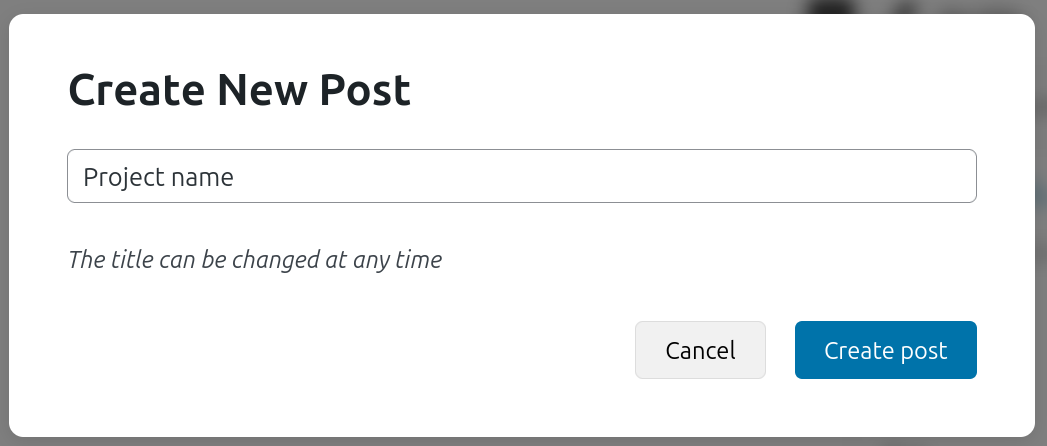
\includegraphics[width=.7\linewidth]{Image/Process/Name.png}
        \caption{Give it a Name}
        \label{fig:name}
    \end{subfigure}
    \bigskip
    %\vspace{.1cm}
    \begin{subfigure}[b]{\textwidth}
        \centering
        
\includegraphics[width=.7\linewidth]{Image/Process/upload.png}
        \caption{Final render}
        \label{fig:first_upload}
    \end{subfigure}
    \caption{Create the post}
\end{figure}

\newpage
\subsection*{Update the settings of the Post}\label{ssec:settings}
\begin{enumerate}
    \item Open the [Settings of the Post] > Click [Post] > Upload the image using [Set featured image] (Fig \ref{fig:featured_image})
    \item Copy the Abstract
    \item Click [Add an excerpt...] > Paste the Abstract (Fig \ref{fig:excerpt})
    \item Click on the Slug > Change it to project-{ID} with the ID of the project (Fig \ref{fig:slug})
    \item The settings should then look like Figure \ref{fig:final_settings}
\end{enumerate}
\

\begin{figure}[h!]
    \centering
    \begin{subfigure}[b]{0.4\textwidth}
        \centering
        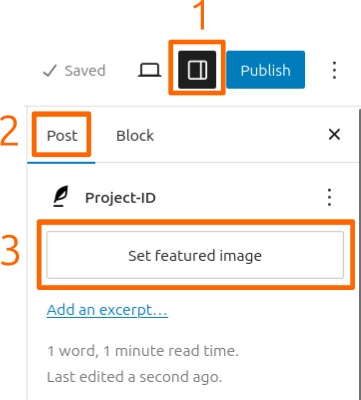
\includegraphics[width=\textwidth]{Image/Process/featured_image.png}
        \caption{Set featured image}
        \label{fig:featured_image}
    \end{subfigure}
    \hfill
    \begin{subfigure}[b]{0.4\textwidth}
        \centering
        
\includegraphics[width=\linewidth]{Image/Process/excerpt.png}
        \caption{Change excerpt}
        \label{fig:excerpt}
    \end{subfigure}
    \bigskip
    \vspace{.1cm}
    \begin{subfigure}[b]{0.6\textwidth}
        \centering
        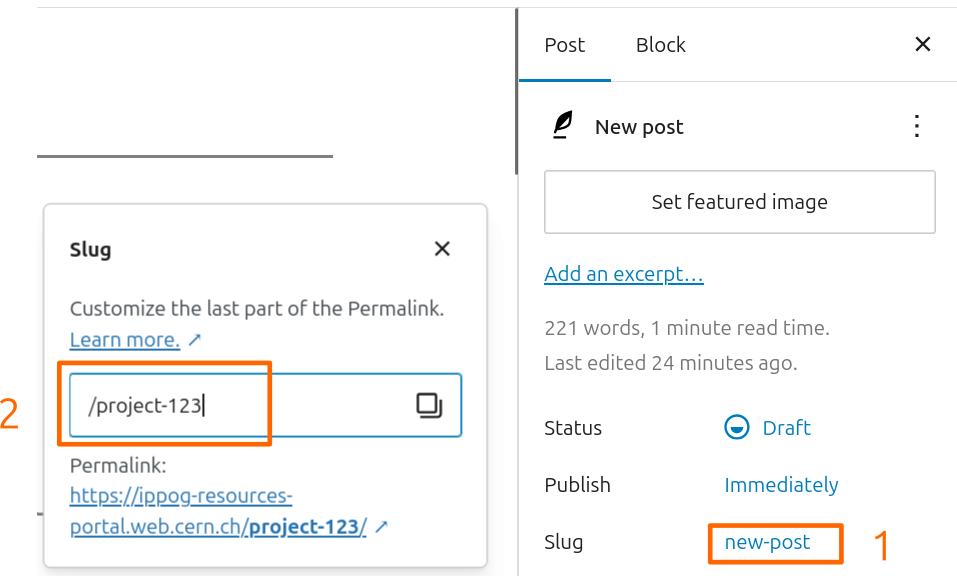
\includegraphics[width=\textwidth]{Image/Process/slug.png}
        \caption{Change the slug}
        \label{fig:slug}
    \end{subfigure}
    \hfill
    \begin{subfigure}[b]{0.3\textwidth}
        \centering
        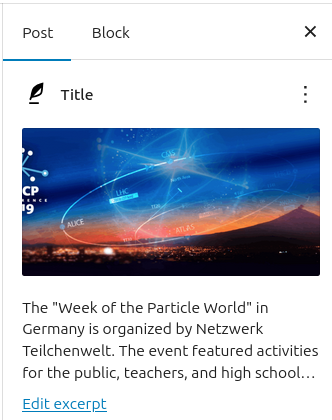
\includegraphics[width=\linewidth]{Image/Process/final_settings.png}
        \caption{Final settings render}
        \label{fig:final_settings}
    \end{subfigure}
    \caption{Settings}
\end{figure}

\newpage
\subsection*{Format the title field}\label{ssec:title}
\begin{enumerate}
    \item Create a block \gray{/media \& text} 
    \item Select [Use featured image] > [Show media on the right] (\ref{fig:media_text})
    \item Create a block \gray{/Title} on the left text field and choose [H1 size]
    \item (optional) Write the subtitle in [H2 size] if there is one
    \item Put the Credit text [aligned right]
    \item Remove all the text beginning with [draft] (\ref{fig:title_final})
\end{enumerate}
\

\begin{figure}[h]
    \centering
    \begin{subfigure}[b]{\textwidth}
        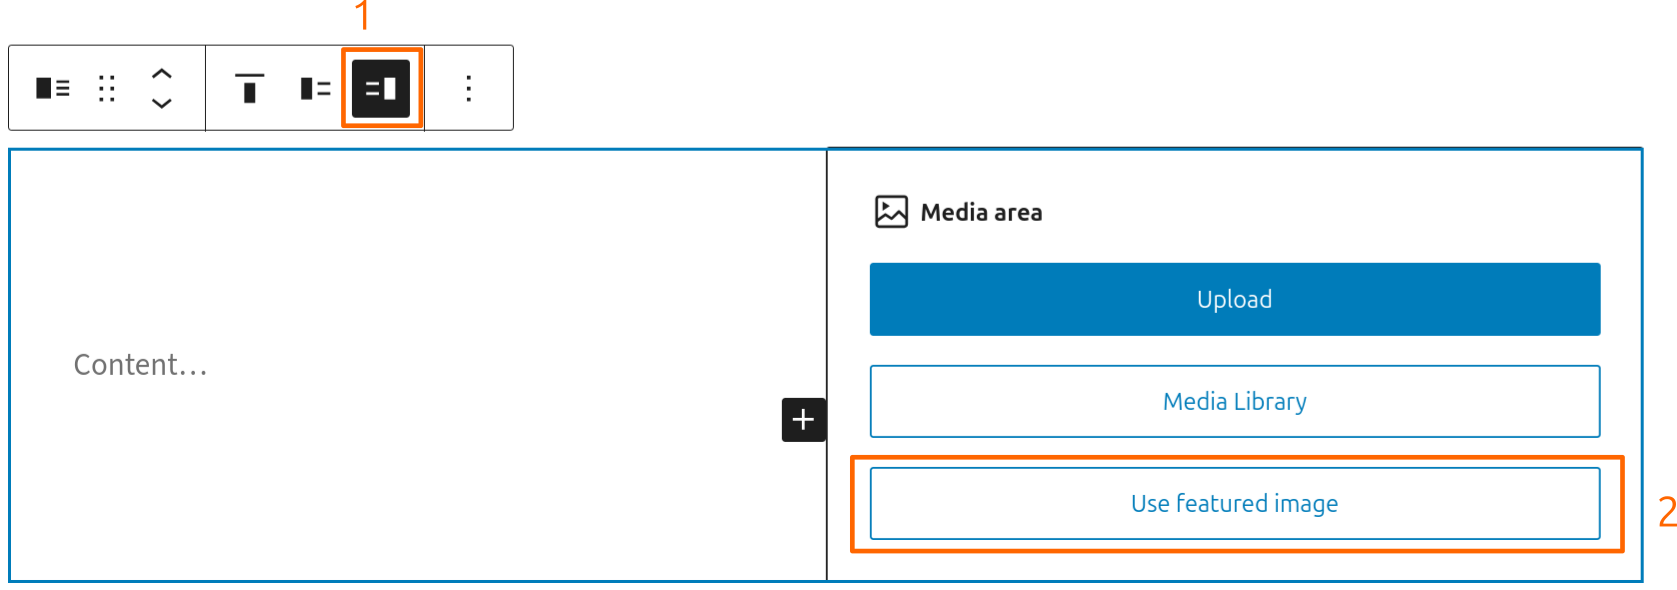
\includegraphics[width=\linewidth]{Image/Process/media_text.png}
        \caption{Media \& Text block}
        \label{fig:media_text}
    \end{subfigure}
    \bigskip
    \vspace{.1cm}
    \begin{subfigure}[b]{\textwidth}
        \centering
        
\includegraphics[width=\linewidth]{Image/Process/title_final.png}
        \caption{Final rendering of the title field}
        \label{fig:title_final}
    \end{subfigure}
    \caption{Title field}
\end{figure}

\newpage
\subsection*{Complete the categories and tags field}\label{ssec:categories}
\begin{enumerate}
    \item Create blocks \gray{/categories} and \gray{/tags}
    \item Respectively add "Categories: " and "Tags: " as prefixes (Fig \ref{fig:tags_categories})
    \item Open the [Settings of the Post] > Click [Post] > Remove "Miscellaneous" and complete the missing tags and categories (Fig \ref{fig:tags_categories_settings})
    \item Remove all the text beginning with [draft]
    \item Change the length of Separators to wide
    \item Finally, publish the article as it is (Fig \ref{fig:publish})
\end{enumerate}

\begin{figure}[th]
    \begin{subfigure}[c]{.5\textwidth}
        \centering
        \begin{subfigure}[t]{\textwidth}
            \centering
            
\includegraphics[width=.7\textwidth]{Image/Process/tags_categories.png}
            \caption{Tags and Categories display}
            \label{fig:tags_categories}
        \end{subfigure}
        
             
        \vspace{5cm}
        \begin{subfigure}[b]{\textwidth}
            \centering
            
\includegraphics[width=.7\textwidth]{Image/Process/publish.png}
            \caption{Publish the Post}
            \label{fig:publish}
        \end{subfigure}
    \end{subfigure}
        \hfill  % NOTE1: hfill moves horizontally stacked objects as far apart as it can
    \begin{subfigure}[c]{.4\textwidth}
        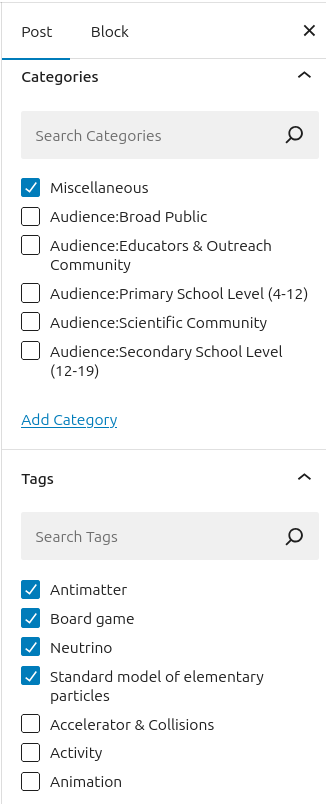
\includegraphics[width=\textwidth]{Image/Process/tags_categories_settings.png}
        \caption{Tags and Categories settings}
        \label{fig:tags_categories_settings}
    \end{subfigure}
    \caption{Uploading the projects}
\end{figure}
\chapter{Data visualization}\label{chap:data}

To visualize the data more easily, multiple tools were developed. An infographic displaying the relationships between tags and categories is created using FraMindmap (Sec. \ref{sec:map}) and pie charts (Sec. \ref{sec:camembert}) are plotted using Python code to visualize the diversity of projects uploaded on the website. 

\section{Types \& Topics map}\label{sec:map}

The mind-map that links tags with their categories (Fig. \ref{fig:Topics_category} \& \ref{fig:Types_category}) is available in FraMindmap\footnote{FraMindmap Types \& Topics taxonomy: \href{https://framindmap.org/c/maps/1527084/edit}{https://framindmap.org/c/maps/1527084/edit}} (Fig. \ref{fig:framamindmap}). It can be easily downloaded as an SVG file or a PNG. A global taxonomy is also available\footnote{FraMindmap Global taxonomy: \href{https://framindmap.org/c/maps/1531458/edit}{https://framindmap.org/c/maps/1531458/edit}}.

/!\textbackslash \ To modify the mind-map, an account is needed. At the moment this document is written, no better alternative was found.

\begin{figure}[h!]
    \centering
    
\includegraphics[width=\linewidth]{Image/Data visualization/framamindmap.png}
    \caption{Framindmap soft}
    \label{fig:framamindmap}
\end{figure}

\newpage
\section{Data visualization}\label{sec:camembert}

The code is available in GitHub: 
\begin{lstlisting}[language=Python]
    git clone https://github.com/Troy314/IPPOG_Website.git
\end{lstlisting}

\begin{itemize}
    \item \gray{data\_topics\_dictionary.py}, \gray{data\_types\_dictionary.py}, \gray{data\_representatives\_dictonary.py} are dictionaries that count respectively the topics and types of the projects as well as the IPPOG members related to each project. 
    \item \gray{data\_analysis\_local.py} \& \gray{data\_analysis\_online.py} files are the codes that create the graphs. They go through all items of the database of which [Status = "Online"] and display pie charts online projects.
    \item \gray{media/data} is the folder where graphs are saved as SVG files
\end{itemize}


Two versions of the code are available
\begin{itemize}
    \item \gray{data\_analysis\_local.py}: directly extract data through Google's API (need the optional dependencies)
    \item \gray{data\_analysis\_online.py}: extract data from a local CSV file 
\end{itemize}

\begin{multicols}{2}
    \raggedcolumns
    \subsubsection*{Online mode}
        
        /!\textbackslash \ Requires the use of Google API, see Sec. \ref{ssec:API}.\newline
        /!\textbackslash \ Requires optional dependencies, see Sec. \ref{dependencies}\newline
        /!\textbackslash \ The JSON file should be put in the same folder as the run file
            
        To run the program, simply run
        \begin{lstlisting}[language=Python]
        python3 data_analysis_online.py\end{lstlisting}
        \columnbreak
    \subsubsection*{Local mode}
        
        /!\textbackslash \ Requires to download the database available on Google sheet\footnote{Google Sheet: \href{https://docs.google.com/spreadsheets/d/1x_SdxdlHwG8chH77WqrTAAgijY2XBY3nPIi2p3TKqzs/edit?gid=1297224389\#gid=1297224389}{https://shorturl.at/sHBrz}} as a CSV file\newline
        /!\textbackslash \ The CSV file should be put in the same folder as the run file
        
        To run the program, simply run
        \begin{lstlisting}[language=Python]
        python3 data_analysis_local.py\end{lstlisting}
        
        The codes will then ask for the name of the CSV file containing the database.
\end{multicols}

The codes produce a \gray{media/data/} folder in which three SVG files are produced: 
\begin{itemize}
    \item Related members data (Fig. \ref{fig:members})
    \item Topics data (Fig. \ref{fig:topics})
    \item Types data (Fig. \ref{fig:types})
\end{itemize}
\chapter{Useful Links}\label{chap:links}

Github Repository with all Python codes, media files, and Guidelines: 
\begin{itemize}
    \item \href{https://github.com/Troy314/IPPOG_Website}{https://github.com/Troy314/IPPOG\_Website}
\end{itemize}

\vspace{.1cm}

Google form that collects the raw data: 
\begin{itemize}
    \item Public: \href{https://docs.google.com/forms/d/e/1FAIpQLSckjdwv7daQZ8jv7D1wwx6mKeZo2Hp4hLGGmV8FT0VTthvOUg/viewform}{https://shorturl.at/Ngf21}
    \item For edition: \href{https://docs.google.com/forms/d/1DzX_IVaZAFX2ucAGyAKSgnYTvkAhOj0lDurSGn4De4E/edit?usp=send_form}{https://shorturl.at/gtkGW}
\end{itemize}

\vspace{.1cm}

Google sheet which hosts the raw database:
\begin{itemize}
    \item \href{https://docs.google.com/spreadsheets/d/1x_SdxdlHwG8chH77WqrTAAgijY2XBY3nPIi2p3TKqzs/edit?gid=1297224389#gid=1297224389}{https://shorturl.at/sHBrz}
\end{itemize}

\vspace{.1cm}

Taxonomy graph available on FraMindmap app:
\begin{itemize}
    \item Public: \href{https://framindmap.org/c/maps/1527084/public}{https://framindmap.org/c/maps/1527084/public}
    \item For edition: \href{https://framindmap.org/c/maps/1527084/edit}{https://framindmap.org/c/maps/1527084/edit}
\end{itemize}

\vspace{.1cm}

IPPOG Websites:
\begin{itemize}
    \item Resource database: \href{https://ippog-resources-portal.web.cern.ch/}{https://ippog-resources-portal.web.cern.ch/}
    \item General Website: \href{https://ippog.org/}{https://ippog.org/}
\end{itemize}

\vspace{.1cm}

Contact:
\begin{itemize}
    \item \href{mailto:Claire.Adam.Bourdarios@cern.ch}{Claire.Adam.Bourdarios [at] cern.ch}
\end{itemize}


\end{document}
